% !TEX root = ../thesis-example.tex
%
\chapter{Algorithmes interactifs / software}
\label{ch:algorithms}

\cleanchapterquote{One general effect of the digital revolution is that avant-garde aesthetic strategies became embedded in the commands and interface metaphors of computer software. In short, the avant-garde became materialized in a computer.}{Lev Manovitch}{The language of the new media}


\noindent La citation de Lev Manovitch en exergue de ce chapitre en reflète la question centrale: le code est l'élément définissant le fonctionnement d'un \gls{DMI} et si sa nature virtuelle rend son usage très malléable, la nature des objets virtuels que l'on manipule est en grande partie conditionnée par les représentations que l'on se fait de l'interaction musicale. Cependant, les machines ont aussi leurs contraintes, leurs limitations et leur hérédité, qui influencent la conception des protocoles et les choix d'implémentation. Après avoir présenté le contexte informatique dans lequel s'inscrivent les développements logiciels d'informatique musicale temps-réel, je détaillerai trois développements en lien avec ces questions :
\vspace{-1em}
\begin{itemize}[noitemsep]
	\item \textbf{le concept de ``modèle intermédiaire dynamique''}, qui au-delà des questions de mise en relation de variables, propose un modèle abstrait pour l'interaction geste/son;
	\item \textbf{le protocole MP}, qui propose une solution alternative au \gls{MIDI} pour répondre aux questions d'agencement et de connexions de modules de traitement, en prenant en compte l'aspect polyphonique en particulier;
	\item \textbf{la librairie \textit{Sagrada}}, qui propose un système original de synthèse granulaire modulaire dans Max contrôlée de manière synchrone ou asynchrone.
\end{itemize}

%%%%%%%%%%%%%%%%%%%%%%%%%%%%%%%%%%%%%%%%%
\section{Matériaux numériques}
\label{ch:algorithms:digital-material}

\subsection{Le son synthétique}

\noindent \iquote{Mais ces instruments numériques que vous fabriquez, ils utilisent des sons enregistrés ou des sons de synthèse ?} Cette question fréquemment posée par des interlocuteurs curieux des nouvelles lutheries est révélatrice des catégorisations opérées sur les matériaux et processus à l'œuvre dans les instruments numériques. Elle se traduisent, en termes esthétiques, par des genres musicaux différents dans les musiques actuelles (``field recording'', ``sampling'', ``folk acoustique'', par opposition à ``techno'', ``glitch'', ``musique électronique'') qui reflètent cette distinction que l'on fait intuitivement entre une image \textit{analogique} des sons du monde ``réel'' et les artéfacts \textit{synthétiques} de la machine, quand bien même les deux seraient produits à l'aide d'un ordinateur.\\
\indent Rappelons donc tout d'abord ce préalable: les sons produits par un ordinateur sont tous des sons de synthèse.\\
\indent On viendra opposer à ce postulat la nature plus artificielle d'un son purement créé à partir d'une équation mathématique, tel un son de synthèse FM, par rapport à la relecture d'un enregistrement audio réalisé à partir d'une source acoustique. Pourtant, la relecture de cet enregistrement n'est, du point de vue de son fonctionnement technique, guère différente de la lecture d'une table d'onde dans une synthèse additive. À la différence perceptive du résultat vient donc s'opposer une évidente parenté de moyens. De plus, les lutheries numériques, en pratique, reposent moins sur des modèles théoriques purs que sur des formes hybrides. Si l'on utilise un enregistrement audio-numérique, cela ne sera généralement pas pour le reproduire tel quel, inchangé, mais pour en jouer, en utilisant le processus de lecture comme un algorithme interactif, avec ses variables paramétriques de vitesse de lecture, de position, de gain, etc.

\subsection{Contrôle de la synthèse, synthèse du contrôle}

\noindent En paraphrasant Edgar Varèse qui décrivait la musique comme \textit{l'art des sons organisés}, on pourrait donc dire que le son numérique est l'art des bits organisés. Sans descendre aussi profondément dans le fonctionnement technique de la machine et son alphabet binaire, on peut considérer, d'un point de vue fonctionnel, que la partie numérique d'un \gls{DMI} est composée de deux grands types de données :
\vspace{-1em}
\begin{itemize}[noitemsep]
	\item \textbf{le code}, ou comme le dirait Bernard Stiegler les ``rétentions tertiaires'', qui prennent la forme d'algorithmes ou de structures de données;
	\item \textbf{les flux}, provenant des capteurs de l'interface, du réseau, ou du code lui même, dans sa capacité à les auto-générer, et qui se modifient en ``traversant'' le code pour produire \textit{in fine} des signaux audio.
\end{itemize}
\noindent Dans les environnements de programmation audio, on opère généralement une distinction entre deux types de flux de données : 
\vspace{-1em}
\begin{itemize}[noitemsep]
	\item \textbf{des signaux synchrones}, représentant par exemple des signaux audio, échantillonnés à une fréquence précise, et traités généralement par bloc dans un \gls{DSP};
	\item \textbf{des événements asynchrones}, arrivant de manière sporadique, tels que les messages \gls{MIDI}, \gls{OSC} ou d'autres types de messages propres au programme et traités dans un graphe de contrôle réactif;
\end{itemize}

\noindent Si cette distinction reflète une différence ontologique entre le domaine du continu et celui du catégoriel, ces deux types de flux traduisent également deux granularités temporelles différentes et sont généralement associés aux notions d'\textit{audio-rate} et de \textit{control-rate}\footnote{On retrouve cette distinction dans tous les logiciels basés sur l'utilisation du \gls{MIDI}, mais également dans Max, dans SuperCollider, dans Csound et même dans Chuck qui permet pourtant que le contrôle soit cadencé à une fréquence arbitraire aussi élevée, voire plus, que celle de l'échantillonage audio.}. Il est intéressant de noter que le contrôle est ainsi implicitement défini comme un signal sporadique et de fréquence moindre que le signal audio-numérique, ce qui relève en soi d'une représentation musicale qui pourrait être discutée.\\
\indent Ainsi, le signal numérique (synchrone) se présente souvent comme l'image d'un signal (audio) analogique échantillonné, avec l'idée de continuité qui lui est associée, tandis que les messages asynchrones se présentent souvent comme l'image d'un ordre d'éxecution (e.g. une note-on \gls{MIDI}). D'un côté, nous avons un signal continu et mono-dimensionnel (un seul échantillon est traité à la fois), de l'autre un signal sporadique et potentiellement polyphonique (plusieurs messages peuvent être envoyés au même instant logique, sans qu'ils soient associés à des flux différents).\\
\indent Cependant, du point de vue de leur usage, les frontières entre ces deux types de données numériques d'une part, et ces deux natures d'objets conceptuels (le signal continu et l'ordre événementiel) d'autre part, ne se recouvrent pas exactement. Il est ainsi courant d'utiliser des messages asynchrones pour convoyer des variables continues (telles que les données d'un contrôle MIDI-CC ou d'un capteur envoyé par \gls{OSC}). À l'inverse, il est également possible d'utiliser un signal synchrone pour déclencher des événements (musicaux) discrets. C'est par exemple le cas lors qu'on envoie une impulsion dans une synthèse de type \gls{KarplusStrong}, ou pour déclencher une enveloppe ou la lecture d'un échantillon\footnote{comme c'est le cas dans le système de synthèse granulaire Sagrada, présenté en section\ref{sec:algorithms:sagrada}}.

\indent Par ailleurs, la programmation des \glspl{DMI} adopte souvent un paradigme de \textit{dataflow}, telle que la programmation ``réactive'', pour répondre aux besoins du temps-réel, tout en s'intégrant dans un environnement multi-paradigmes\footnote{Un logiciel tel que Max qui s'articule essentiellement autour d'une programmation visuelle de \textit{dataflow}, intègre également des possibilités de scripting, de programmation synchrone, fonctionnelle ou impérative.}. Une autre distinction qui en découle en partie, est celle qui consiste à séparer les algorithmes de synthèse audio d'une part, et le \textit{mapping}\footnote{c'est-à-dire les relations --~potentiellement algorithmiques~-- entre les ``entrées'' de l'instrument (telles que les données issues d'une interface sensible\footnote{Sur la notion d'interface sensible, cf. \ref{ch:interfaces}}) et la synthèse. Cf. section \ref{sec:algorithms:MID:mapping-to-MID} d'autre part en deux objets conceptuels distincts, comme en témoignent les représentations de modèles de mappings proposés sur les figures \ref{fig:algorithms:DynamicMappingLayer1}, \ref{fig:algorithms:DynamicMappingLayer2}, \ref{fig:algorithms:DynamicMappingLayer3}}.\\
\indent Si ces différentes distinctions résultent de contraintes techniques, d'évolutions historiques, de choix conceptuels voire d'intentions musicales, j'ai cependant choisi de regrouper dans ce chapitre des aspects concernant à la fois le mapping et la synthèse. Ce choix est motivé par la porosité évidente qu'il existe entre ces différentes catégories et par des développements qui tentent, en partie, de redéfinir leur articulation.


\subsection{Modèles [psycho]acoustiques}
Intégration dans les algorithmes de modèles décrivant la réalité qui nous entoure, pour simuler le réel par des stimulus trompant notre perception. (cf. gestes subversifs)
Eg. modélisation de la résonance des matériaux, des lieux (eg. logiciels de spat)
modélisation de la perception du son (eg. effet doppler, compression pumping)
modèle musicaux (gammes et accords, arpeggiateur)

\subsection*{[Extra material]}

Jorda : \iquote{The most direct kind of mapping, which associates each single sound control parameter (e.g., pitch, amplitude, etc.) with an independent control dimension, has proved to be musically unsatisfying, exhibiting a toy-like characteris- tic that does not allow for the development of virtuosity. More complex mappings, which, depending on the type of relation between inputs and synthesis parameters are usually classified as one-to-many, many-to-one or many-to-many, have proven to be more musically useful and interesting (Hunt, 1999; Hunt, Wanderley, Kirk, 2000).}

Et d'un autre côté : il faut un mapping causal et on cherche à mapper un capteur sur un paramètre musical (Cadoz, Vertegaal)



L’atomisation jusqu’au sample, plutôt que séparation entre DSP et messages de contrôle
=> faust, gen\textasciitilde{ } et cie : l’export vers des plateformes multiples.\\
\indent D'après Hunt et Wanderley \cite{hunt_mapping_2002}, deux directions dans le design de mapping :
\vspace{-1em}
\begin{itemize}[noitemsep]
	\item \textbf{generative mechanisms}, such as neural networks to perform mapping;
	\item \textbf{explicitly defined mapping strategies}.
\end{itemize}
Exemples de schéma de mapping de Wanderley dans \cite{wanderley_escher-modeling_1998}.\\
MnM : \cite{bevilacqua_mnm_2005}\\
``complex mappings are more satisfactory, after a learning phase, than one-to-one mapping'' in \cite{wanderley_mapping_2002}\\
\extra{\cite{hunt_mapping_2002}: \iquote{(...) we define mapping as the act of taking real-time performance data from an input device and using it to control the parameters of a synthesis engine.}}
Sound is the interface, \cite{di_scipio_sound_2003}


%%%%%%%%%%%%%%%%%%%%%%%%%%%%%%%%%%%%%%%%%
\section{Modèles intermédiaires dynamiques}
\label{sec:algorithms:MID}

\subsection{Du mapping aux modèles intermédiaires dynamiques}
\label{sec:algorithms:MID:mapping-to-MID}

\subsubsection{Origines du terme mapping} 

\noindent Dans le domaine des lutheries numériques, le terme de ``mapping'' est très couramment utilisé pour décrire la relation entre les données issues des capteurs de l'interface sensible et les paramètres de la synthèse sonore. Le terme lui-même est issu des mathématiques dans lequel il se traduit en français par ``application'', c'est-à-dire une relation entre deux ensembles pour lequel chaque élément du premier (appelé ensemble de départ) est relié à un unique élément du second. Andy Hunt le définit ainsi comme \iquote{la liaison ou la correspondance entre les paramètres de contrôle (dérivés des actions de l'interprète) et les paramètres de synthèse sonore}\footnote{``the liaison or correspondence between control parameters (derived from performer actions) and sound synthesis parameters'' \cite{hunt_towards_2000}}.\\
\indent Ce terme a glissé dans le vocabulaire de la lutherie numérique en raison de la relative simplicité des relations de correspondance dans les premiers \glspl{DMI} et est resté, alors que ces relations se sont progressivement complexifiées, comme le notait déjà Joel Chadabe en 2002 : \iquote{Le mapping décrit la façon dont un contrôle est connecté à une variable. Mais à mesure que les instruments deviennent de plus en plus complexes pour inclure de grandes quantités de données, une sensibilité au contexte, ainsi que des capacités de génération sonore et musicale, le concept de mapping devient plus abstrait et ne décrit pas les réalités plus complexes des instruments électroniques}\footnote{Mapping describes the way a control is connected to a variable. But as instruments become more complex to include large amounts of data, context sensitivity, and music as well as sound-generating capabilities, the concept of mapping becomes more abstract and does not describe the more complex realities of electronic instruments. \cite{chadabe_limitations_2002}}.

\subsubsection{Un grand répertoire}

\noindent Le \textit{mapping} est un domaine en effervescence depuis le début des années 2000 et de nombreusx modèles ont été proposés (figures \ref{fig:algorithms:DynamicMappingLayer1}, \ref{fig:algorithms:DynamicMappingLayer2}, \ref{fig:algorithms:DynamicMappingLayer3}), passant la proposition de modèles multi-couches (\cite{wanderley_escher-modeling_1998, hunt_mapping_2002}), auto-adaptatifs \cite{verfaille_mapping_2006}, de cartographie de paramètres sur des espaces perceptifs (\cite{wessel_timbre_1979, schwarz_sound_2012, tubb_divergent_2014}), de métaphores d'interaction avec des objets virtuels (\cite{wessel_intimate_2002}), de projections des paramètres de synthèse sur des espaces perceptifs (\cite{wyse_instrumentalizing_2010}), de modèles physiques ou visuels (\cite{momeni_dynamic_2006}), de modèles géométriques (\cite{van_nort_choice_2004}), stochastiques (\cite{dabby_musical_1996}), d'apprentissage automatique basé sur la corrélation entre le geste et le son (\cite{fiebrink_real-time_2011, caramiaux_mapping_2014, francoise_motion-sound_2015}).\\
\indent À cette longue liste s'ajoute celle, probablement plus longue encore, de mappings empririques qui ont émergés lors de la conception expérimentale de nouveaux \glspl{DMI} et qui n'ont pas été identifiés, nommés ou présentés de manière formelle dans une conférence académique.

\subsubsection{La qualité d'un mapping est contextuelle}

\noindent Ces différentes approches relèvent (sans que cela soit nécessairement exprimé explicitement par leurs auteurs) de dynamiques différentes concernant l'interaction musicale et ses finalités. Ainsi, plusieurs études ont été publiées, tentant de cerner les contours de la notion de mapping, de les catégoriser et de les comparer qualitativement. Cependant, si certains de ces articles ont tenté de montrer que certains types de mappings fonctionnaient mieux que d'autres, il semble difficile de les évaluer en dehors du cadre spécifique dans lequel ils ont été conçus\footnote{...et nous avons vu dans le chapitre \ref{ch:gesture} la diversité des situations d'interaction musicale, allant de la composition à la performance, en passant par des situations d'écoute, de pédagogie, etc.}, et encore moins dans la perspective d'une ``universalité'' --~qui semblerait aujourd'hui davantage être une ``\textit{multiversalité}''. Leur qualité est en effet extrêmement complexe à évaluer et fait intervenir, au-delà du modèle théorique qui les régit, la qualité des capteurs, la fréquence d'échantillonnage, le type de synthèse contrôlée en aval, les conditions environnementales (qui peuvent altérer la manière dont le geste est capté), les motivations musicales sous-jacentes, et par suite, des considérations esthétiques éminemment subjectives\footnote{Par exemple, les assertions prétendant qu'un mapping complexe donnait de meilleurs résultats qu'un mapping simple (\cite{rovan_instrumental_1997, hunt_mapping_2000}) sont facilement invalidables. Sergi Jorda prenait l'exemple du Theremin dans \cite{jorda_digital_2005} pour mettre en évidence le succès d'un mapping \textit{one-to-one}.}.

\subsubsection{Mappings hybrides} 

\noindent Nous sommes ainsi aujourd'hui dans une situation où de nombreuses stratégies de mapping sont disponibles, qui loin de s'exclurent mutuellement, constituent un répertoire très riche pour composer le design de l'interaction instrumentale. En effet, au-delà de l'utilisation de stratégies isolées à des fins démonstratives\footnote{...comme c'est souvent le cas dans les présentations scientifiques et dans les démonstrations qui les accompagnent.}, le design de l'interaction instrumentale est souvent un hybride de différentes stratégies qui se complètent. Par ailleurs, si la plupart des stratégies de mapping présentées dans la littérature cherchent à obtenir une cohérence entre le geste et le son, nous avons vu au chapitre \ref{ch:gesture}, que cette cohérence n'est pas nécessairement une finalité dans la création musicale. La possibilité de mélanger les mappings présentés dans la littérature, de les ``abuser'' et de les ``corrompre'', fait donc partie intégrante du processus d'élaboration de l'interaction instrumentale.\\
\indent Ainsi, malgré sa popularité\footnote{Entre 2001 et 2015, le terme "mapping" a été employé dans plus de 750 articles de la conférence \gls{NIME} alors que "design d'interaction" (interaction design) n'était employé que dans 160 articles.}, le terme de mapping semble assez peu représenter la complexité de ce qui n'est pas une simple mise en relation de paramètres et nous préférerions parler d'un ``design interactif'', c'est-à-dire d'une programmation interactive des relations entre gestes et sons faisant intervenir modèles physiques, d'apprentissage, de mise à l'échelle, de filtrage, des scénarios évolutifs, fragments de partitions, etc. qui s'agencent dans la pratique selon des scénarios complexes (cf. schéma figure \ref{fig:algorithms:DynamicMappingLayer4} et exemple figure \ref{fig:algorithms:FIBR-patch}).\\
\noindent Ce sont ces différents traitements, lorsqu'ils se cristallisent en des agencements identifiables, que l'on peut extraire sous forme d'un modèle abstrait ré-utilisable, que l'on nommera ici ``modèles intermédiaires dynamiques''.

\subsubsection{Extra material}

\cite{momeni_dynamic_2006}, \cite{winkler_making_1995}, 
Toolboxes : ESCHER (Wanderley et al)\cite{wanderley_escher-modeling_1998}, Mapping library for Pd (Steiner) \cite{steiner_towards_2006}, MnM (Bevilacqua et al.) \cite{bevilacqua_mnm_2005}, Libmapper

%------------------ Figure : représentation du mapping #1 #2 ---------------------
\begin{figure}[!htbp]
	\captionsetup{format=plain}%
	\centering
	\begin{minipage}[t]{0.48\textwidth}
		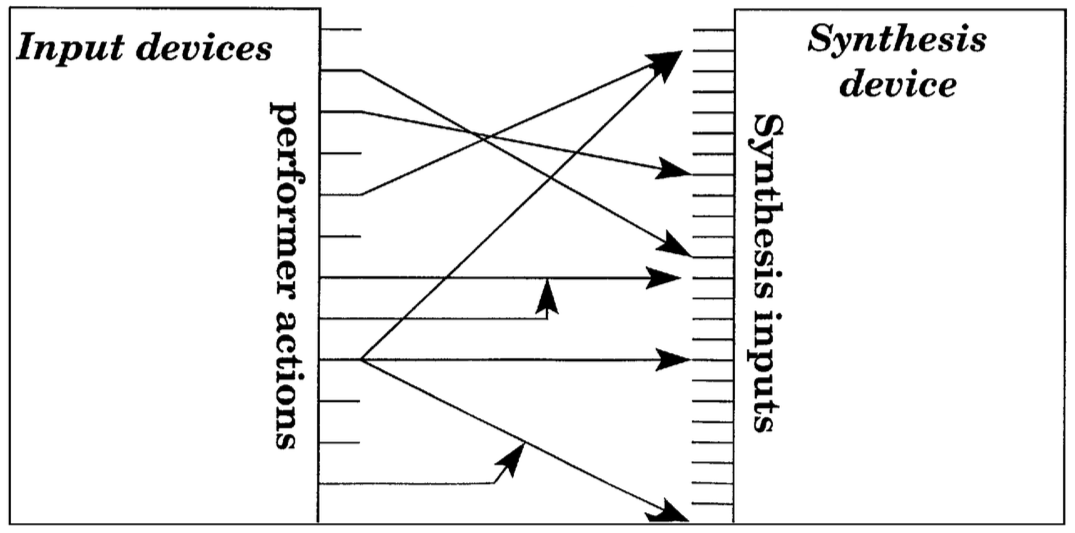
\includegraphics[width=\linewidth]{gfx/04_algorithms/Wanderley_Schema1.png}
		\caption[Représentation du mapping \#1]{Mapping entre contrôleur et synthèse d'après \cite{hunt_towards_2000}}
		\label{fig:algorithms:DynamicMappingLayer1}
	\end{minipage}
	\hspace{.02\linewidth}
	\begin{minipage}[t]{0.48\textwidth}
	  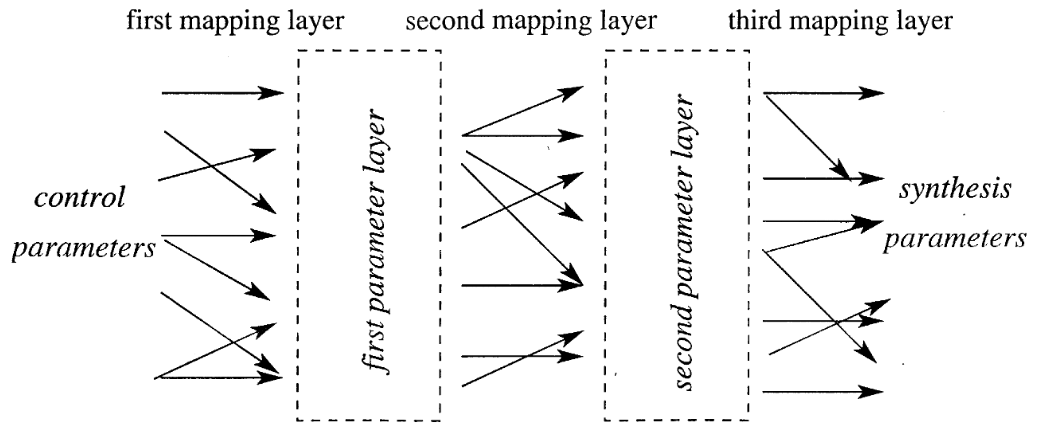
\includegraphics[width=\linewidth]{gfx/04_algorithms/Wanderley_Schema2.png}
		\caption[Représentation du mapping \#2]{Mapping multi-couches d'après \cite{hunt_mapping_2002}}
		\label{fig:algorithms:DynamicMappingLayer2}
	\end{minipage}
\end{figure}
%------------------ Figure : représentation du mapping #1 #2 ---------------------

%------------------ Figure : représentation du mapping #3 #4 ---------------------
\begin{figure}[!htbp]
	\captionsetup{format=plain}%
	\centering
	\begin{minipage}[t]{0.48\textwidth}
	 	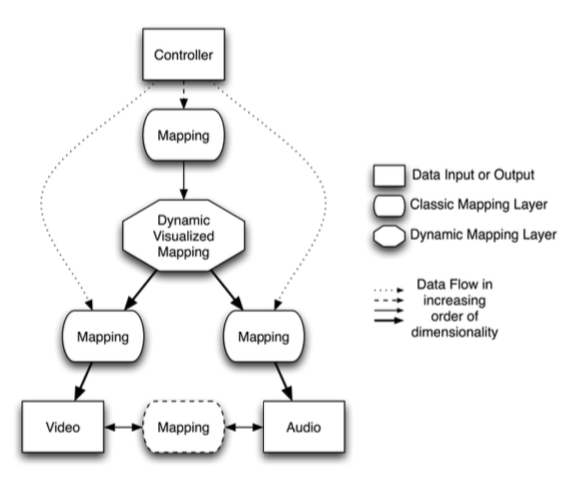
\includegraphics[width=\linewidth]{gfx/04_algorithms/Momeni-DynamicMappingLayers.png}
		\caption[Représentation du mapping \#3]{Mapping intermédiaire dynamique, d'après \cite{momeni_dynamic_2006}}
		\label{fig:algorithms:DynamicMappingLayer3}
	\end{minipage}
	\hspace{.02\linewidth}
	\begin{minipage}[t]{0.48\textwidth}
	  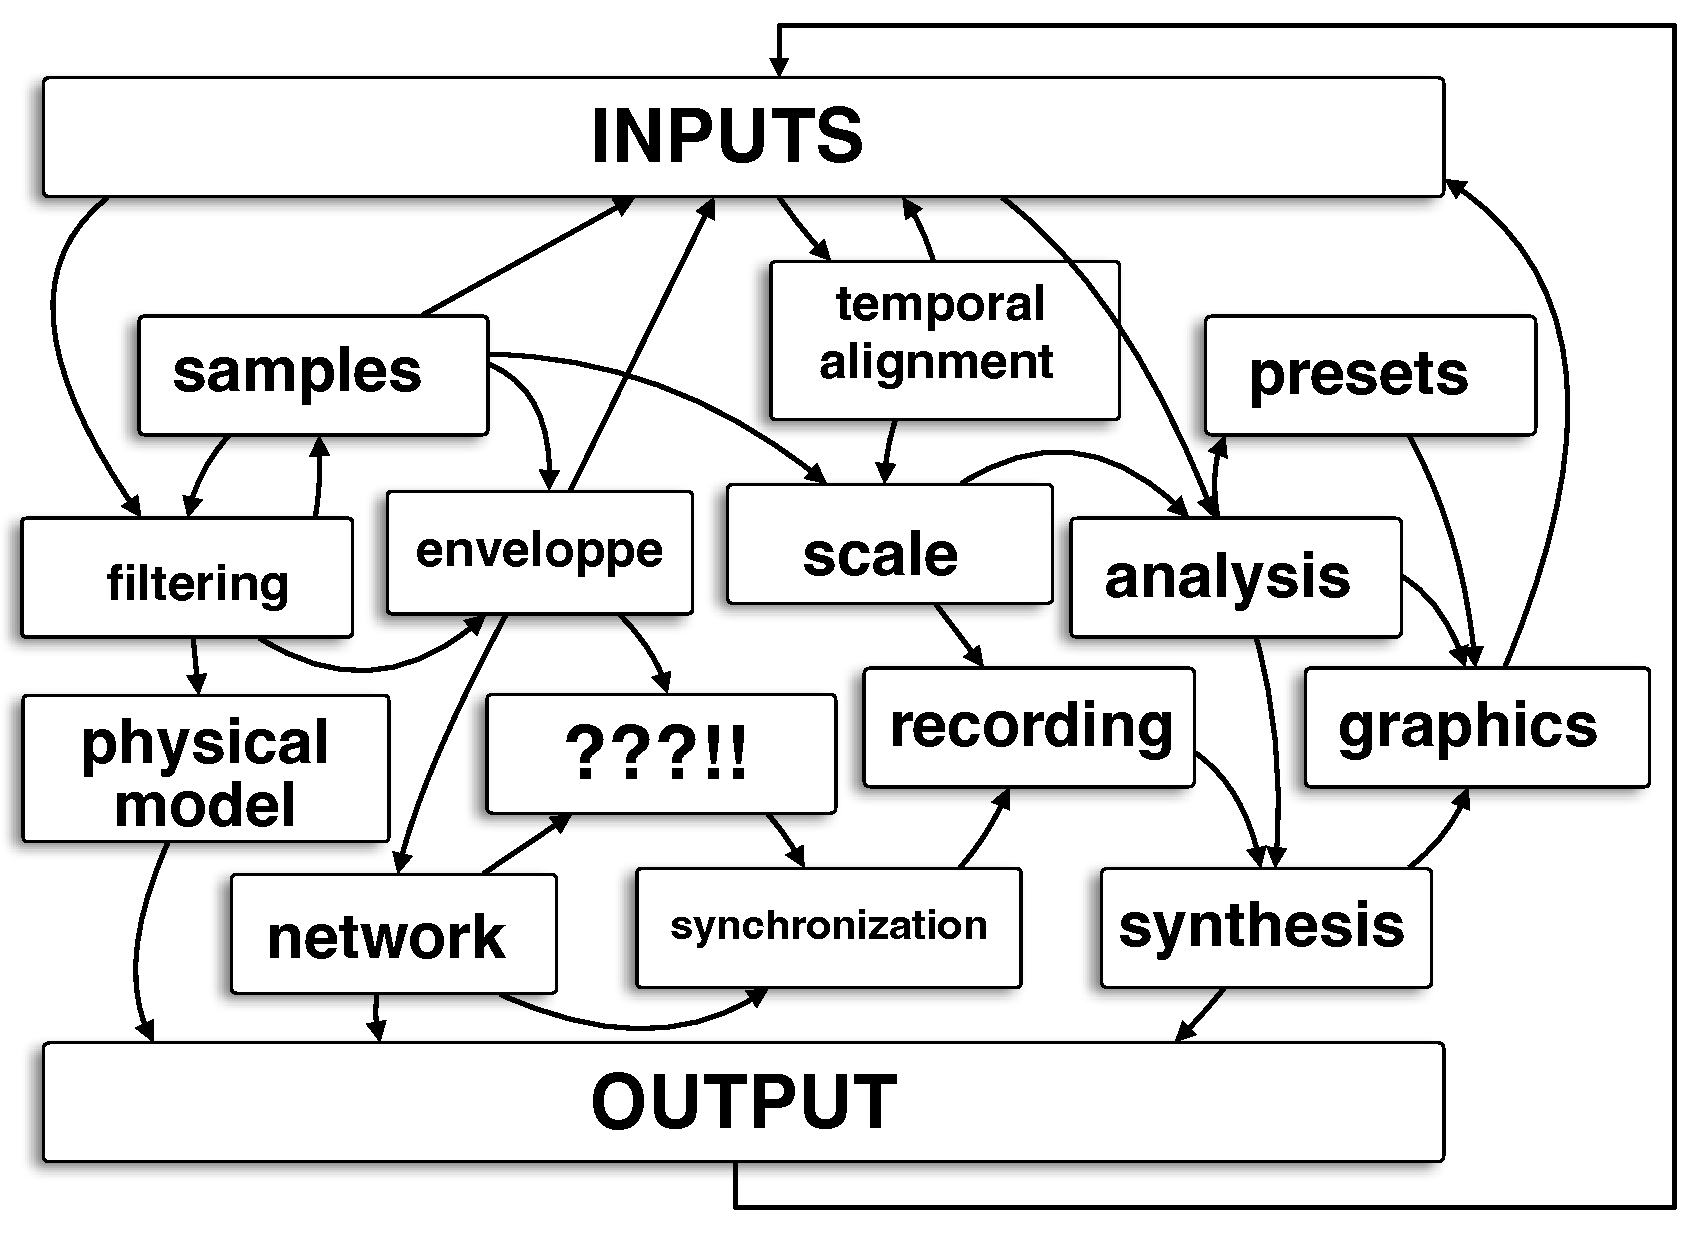
\includegraphics[width=\linewidth]{gfx/04_algorithms/mapping-IRL.pdf}
		\caption[Représentation du mapping \#4]{Mapping, ``dans la vraie vie'' (schéma outrageusement simplifié)}
		\label{fig:algorithms:DynamicMappingLayer4}
	\end{minipage}
\end{figure}
%------------------ Figure : représentation du mapping #3 #4 ---------------------

%------------------ Figure : MID ---------------------
\begin{figure}[!htbp]
	\captionsetup{format=plain}
	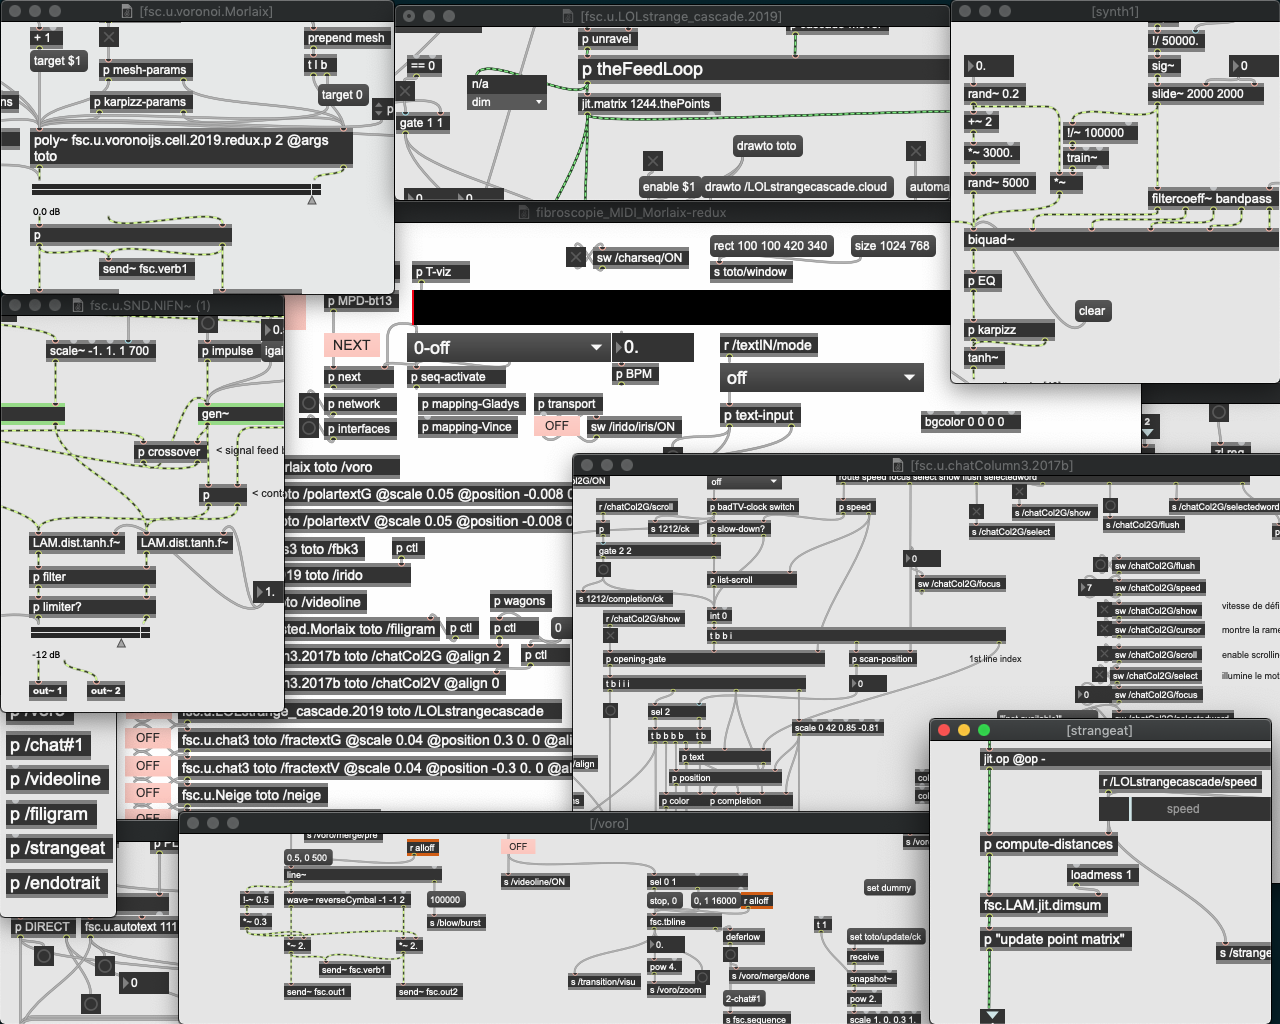
\includegraphics[width=\textwidth]{gfx/04_algorithms/FIBR-patch.png}
	\caption[Aperçu d'un patch Max]{Aperçu partiel du patch Max utilisé dans la performance ``FIB\_R''.}
	\label{fig:algorithms:FIBR-patch}
\end{figure}
%------------------ Figure : MID ---------------------

\subsection{Rôle des modèles intermédiaires}

\noindent Un ``modèle intermédiaire dynamique'', selon notre définition, est un processus de traitement d'un signal apparenté à du geste et qui produit un signal transformé, apparenté, lui aussi, à du geste\footnote{J'utilise l'expression ``apparenté à du geste'' car d'une part, ce signal n'est que son image captée et numérisée, et d'autre part car la frontière entre ce qui est ``geste'', ``image'', ``son'', ... une fois le signal numérisé, est éminemment poreuse.}.\\
\indent Parmi les qualités recherchées lors de l'utilisation de MID, se trouvent en bonne place les qualités que l'on trouve sur les instruments acoustiques, perdues dans leur transposition numérique : finesse et richesse de l'interaction avec des matériaux (frottement, grincement, râclement... et tous les phénomènes subtils et non-linéaires qui se produisent en fonction de l'état de surface, de la viscosité et des propriétés élastico-mécaniques des matériaux). Certains de ces modèles s'inspirent ainsi d'équivalents dans le domaine des instruments acoustiques, qui usent eux aussi de systèmes --~plutôt que de modèles~-- intermédiaires (si l'on considère, par exemple, l'archet comme un système intermédiaire entre le geste du violoniste et la corde). D'autres sont plus spécifiques au numérique, tels que les modèles agissant sur l'aspect temporel du geste ou sur sa reconnaissance.\\
\indent La liste suivante présente plusieurs axes selon lesquels ces modèles affectent le mouvement :
\vspace{-1em}
\begin{itemize}[noitemsep]
	\item \textbf{en qualité}: les MIDs peuvent venir enrichir le mouvement, que cela soit de manière statique, en modifiant sa plage de valeur, ou dynamique, en le modulant pour lui ajouter un contenu fréquentiel absent dans le geste capté, excédant potentiellement les capacités motrices humaines\footnote{Nick Collins présente ainsi son algorithme BBcut: ``\textit{The sort of audio cutting assumed here is usually at haptic or human rhythmic rates, with the obvious capability to reach inhuman speeds.}'' dans \cite{collins_bbcut_2002}}, par exemple, un vibrato, un tremolo, une distorsion, etc. Le champ des possibilités est très vaste, tant la richesse du signal fourni par les capteurs gestuels sur les \glspl{DMI} est généralement bien en deça de la richesse des interactions se produisant dans les instruments acoustiques.\\
	\indent Il est ainsi plus rare, quoique possible, qu'un MID \textit{réduise} la richesse du mouvement. Cela peut cependant se présenter, dans le cas de modèles qui visent à borner son amplitude, ou réduire ses variations. Un exemple notoire dans les musiques pop actuelles est l'\textit{auto-tune} qui vient réduire les variations de hauteur dans la voix naturelle, pour la contraindre sur une hauteur fixe. Dans le cas du geste, le système de quantification dynamique de la hauteur présenté dans \cite{goudard_playing_2014} en est un exemple (cf. figure \ref{fig:algorithms:MID-dynamic-pitch-correction}).\\
	\indent La nature de l'altération vient conférer une identité musicale au modèle intermédiaire, un ``son'' spécifique. Par exemple, l'algorithme BBcut \cite{collins_bbcut_2002} et ses variations\footnote{notamment : \textit{modsquad} (2000) de Atau Tanaka dans Max, \textit{LiveCut} de Rémy Muller, \textit{BeatRepeat}(2005) dans Ableton Live 5} est une signature, qui associée à une famille de boucles rythmiques\footnote{Notamment les ``Amen Break'' des Winstons, ``Funky Drummer'' de James Brown, ``Think'' de Lyn Collins.}, est audible dans toute la musique breakbeat et ``incorpore'' --~pour reprendre l'expression de Manovitch en exergue de ce chapitre~-- les techniques de scratch des DJs et de segmentation de boucles rythmiques re-séquencées dans les boites à rythmes.

	\item \textbf{en quantité}: le geste peut également être augmenté quantitativement, en le démultipliant et en créant une polyphonie à partir d'un mouvement unique. C'est le cas, par exemple, des algorithmes de foule (e.g. algorithme de Boids), ou des modèles physiques qui permettent de générer une multitude de mouvements constituant la réponse d'un matériau virtuel sur lequel on exerce une simple force. Le mouvement peut également être réduit en quantité, notamment par des systèmes de cribles qui ne laissent passer que certaines valeurs.
	
	\item \textbf{dans sa continuité}: les algorithmes permettant de quantifier le mouvement en sont des examples, mais également les algorithmes d'analyse qui permettent la reconnaissance de formes labellisées.
	
	\item \textbf{dans sa temporalité}: les machines permettant l'enregistrement et le temps différé offre de multiples possibilités d'étirer, de contracter, de différer le mouvement, que cela soit sous la forme d'échos, de boucles enregistrées, d'alignement temporel sur une partition (e.g. le système Antescofo) ou sur un motif rythmique (e.g. les ``\textit{grooves}'' dans Ableton Live).

	\item \textbf{dans son contenu}: un geste peut également être le simple déclenchement de processus possédant leurs propres mouvements autonomes, comme cela peut être le cas dans les algorithmes stochastiques ou génératifs (cf. modèle basé sur le ``jeu de la vie'', présenté dans les examples en section \ref{sec:algorithms:MID:examples}). Un autre exemple intéressant est celui du sélecteur de bande radio, qui transforme un simple geste de rotation de potentiomètre en des changements disruptifs de contenus musicaux, tel qu'utilisé par John Cage dans sa pièce ``Imaginary Landscape No. 4'', et qui a été adapté dans un module Eurorack (cf. interview dans l'Annexe \ref{appendix:dumeaux}).

\end{itemize}


\noindent Indépendemment de leur fonctionnement interne, les MIDs présentent également une certaine affordance, qui facilite leur usage au sein d'un agencement instrumental. La liste ci-après résume quelques aspects souhaitables de cette affordance :
\vspace{-1em}
\begin{itemize}[noitemsep]
	\item \textbf{disponibilité} : pouvoir les convoquer et les délaisser à tout instant (i.e. en cours de geste);
	\item \textbf{interconnectibilité} : pouvoir facilement brancher un modèle sur un autre, sans que la nature ou la valeur de leurs signaux ne restreigne \textit{a priori} cette connection;
	\item \textbf{ajustabilité} : pouvoir ajuster les réglages d'un processus durant le temps de jeu, afin d'expérimenter et d'éprouver son fonctionnement de manière perceptive;
	\item \textbf{éditabilité} : pouvoir les éditer, les modifier, les déconstruire, le ré-agencer en variations exportables;
	\item \textbf{réutilisabilité} : pouvoir créer de multiples instances, dans des agencements différents;
	\item \textbf{bidirectionnalité} : le modèle intermédiaire doit pouvoir communiquer dans les deux sens avec l'interface et les autres modèles afin de pouvoir s'ajuster mutuellement (et en particulier, pouvoir se coupler en assurant une continuité des processus internes);
	\item \textbf{abusabilité} : ne pas contraindre arbitrairement les plages de valeurs selon des critères de raisonnabilité \textit{a priori}, afin de laisser l'espace nécessaire à une expérimentation ``hors-normes'' et une relation subversive (sur l'idée de ``geste subversif'', voir la section \ref{sec:gesture:subversion}). Par exemple, il est intéressant de pouvoir utiliser un modèle physique dans un régime incohérent avec la physique réelle.
\end{itemize}


\subsection{Exemples}
\label{sec:algorithms:MID:examples}

%------------------ Figure : MID ---------------------
\begin{figure}[!htbp]
	\captionsetup{format=plain}
	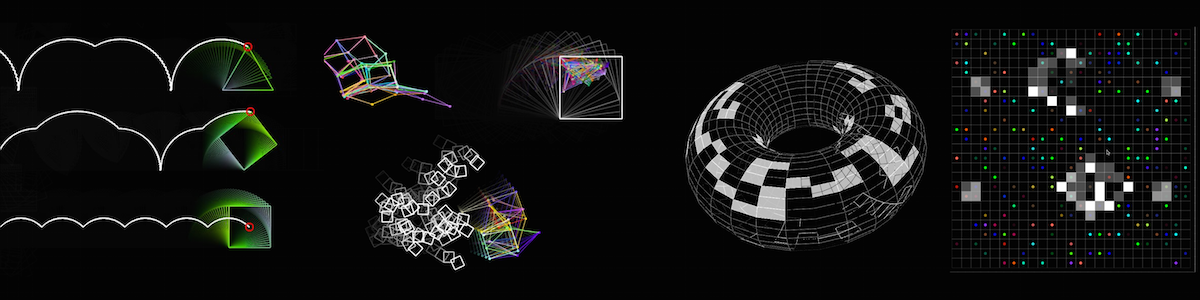
\includegraphics[width=\textwidth]{gfx/04_algorithms/OrJo_MID_1200x300px.png}
	\caption[Modèles intermédiaires dynamiques pour la synthèse audio-graphique]{Modèles intermédiaires dynamiques pour la synthèse audio-graphique. De gauche à droite : a) un modèle géométrique basé sur les courbes cycloïdes, b) un modèle pseudo-physique basé sur l'algorithme de Verlet, c) les modèles de Cycloïdes et de Verlet interconnectés, d) un algorithme génératif basé sur le ``jeu de la vie''.}
	\label{fig:algorithms:MP-MID}
\end{figure}
%------------------ Figure : MID ---------------------

%------------------ Figure : représentation du mapping #3 #4 ---------------------
\begin{figure}[!htbp]
	\captionsetup{format=plain}%
	\centering
	\begin{minipage}[t]{0.48\textwidth}
	 	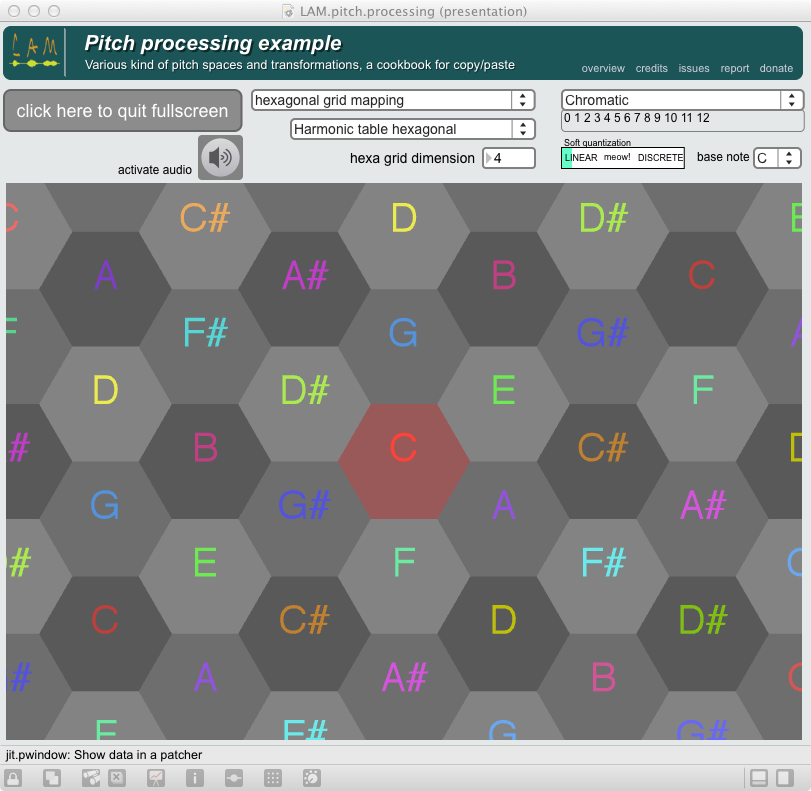
\includegraphics[width=\linewidth]{gfx/04_algorithms/MID-HarmonicHexa-mapping.png}
		\caption[Clavier isomorphique dans Max]{Mapping de clavier isomorphique dans la librairie LAM-lib/mp.TUI.}
		\label{fig:algorithms:MID-hexakeyboard}
	\end{minipage}
	\hspace{.02\linewidth}
	\begin{minipage}[t]{0.48\textwidth}
	  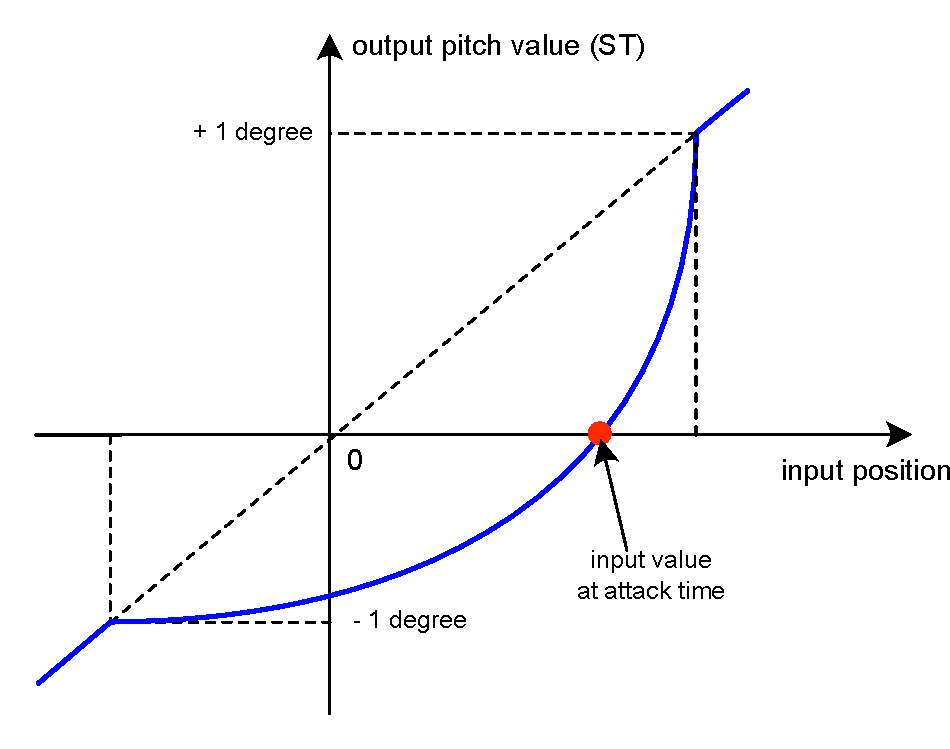
\includegraphics[width=\linewidth]{gfx/04_algorithms/MID-dynamic-pitch-correction.pdf}
		\caption[Correction dynamique de la hauteur]{Correction dynamique de la hauteur à l'attaque de note par anamorphose de la surface de jeu.}
		\label{fig:algorithms:MID-dynamic-pitch-correction}
	\end{minipage}
\end{figure}
%------------------ Figure : MP-event et MP-block ---------------------

\noindent Plusieurs modèles intermédiaires dynamiques ont été développés dans l'équipe \gls{LAM} ces dix dernières années, dans le cadre de plusieurs projets de recherche\footnote{\textit{OrJo} (Orchestre de Joysticks), 2009-2012, projet FEDER, financé par la Région Ile-de-France et \textit{Panam} (Pédagogie Artistique Numérique Accessible et Multimodale ), 2012-2015, projet \gls{ANR}} et donné lieu à des publications, dans la continuité des travaux d'Ali Momeni et Cyrille Henry \cite{momeni_dynamic_2006}, sur le contrôle de modèles audio-graphiques. En particulier, des recherches ont été menées sur les possibilités d'interconnexion de ces modèles\footnote{Une vidéo réalisée durant le projet OrJo donne un aperçu de la manière dont ils peuvent être interconnectés dans un scénario évolutif : \url{https://vimeo.com/25740547}} (figure \ref{fig:algorithms:MP-MID} et voir \cite{goudard_dynamic_2011}). D'autres développements se sont focalisés sur des algorithmes génératifs comme l'automate cellulaire du ``jeu de la vie''\footnote{Une vidéo montre son utilisation dans le logiciel Méta-Mallette : \url{https://vimeo.com/158323394}} (voir \cite{goudard_modeintermediaire_2012}). Enfin, des développements se sont concentrés par l'étude verticale de la gestion du contrôle de la hauteur monophonique \cite{goudard_playing_2014}, en s'intéressant à ses possibles représentations sur une interface bi-dimensionnelle (de type tablette)(figure \ref{fig:algorithms:MID-hexakeyboard}) et sur ses altérations (figure \ref{fig:algorithms:MID-dynamic-pitch-correction}).\\
\indent Ces différents modèles ont été intégrés dans la LAM-lib, un package pour Max librement téléchargeable\footnote{\url{https://github.com/LAM-IJLRA/lam-lib}}. Ils ont notamment été utilisés dans le cadre d'une pratique d'ensemble avec le logiciel Méta-Mallette\footnote{logiciel développé par l'association Puce Muse (\url{https://pucemuse.com})}, ainsi que dans des créations personnelles comme ``FIB\_R''.


%%%%%%%%%%%%%%%%%%%%%%%%%%%%%%%%%%%%%%%%%
\section{MP : polyphonie modulaire et expressive}
\label{sec:algorithms:MP}
%---------------------------------------------------------------------------
\subsection{Une note sur les polyphonies}

\noindent La polyphonie dans les \glspl{DMI} peut être envisagée à plusieurs niveaux: polyphonie de gestes (e.g. plusieurs doigts en contact sur une tablette multitouch), de sons (e.g. plusieurs ``notes'' qui résonnent en même temps) ou de modèles intermédiaires (e.g. plusieurs processus qui tournent en parallèle). Concevoir le design d'un \gls{DMI} poly-poly-polyphonique nécessite par conséquence d'établir les connexions entre ces différentes multiplicités.\\
\indent Les notions de mapping \textit{one-to-one}, \textit{many-to-one}, \textit{one-to-many} et \textit{many-to-many}, telles que définie par \cite{hunt_mapping_2002}, peuvent ainsi s'agencer sur plusieurs niveaux, selon la polyphonie de chaque modèle en jeu, ou être organisées en sous-groupes. Prenons l'exemple de doigts contrôlant chacuns une multiplicité d'agents autonomes, venant chacun contrôler une polyphonie de notes sur une synthèse \gls{FM}. Un scénario souhaitable (c'est un exemple) est que les agents et les notes contrôlés par un même doigt partagent des caractéristiques communes, ce qui nécessite une traçabilité de la source gestuelle jusqu'à la synthèse et/ou un moyen de fusionner les informations nécessaires de part et d'autre des différentes sources concourant au résultat sonore final.\\
\indent Inversement, nous pouvons consider un mapping \textit{many-to-one}, en prenant l'example de plusieurs doigts venant agir sur un même objet virtuel. Dans ce cas, le résultat monophonique produit par l'objet virtuel peut prendre contenir l'information polyphonique des différents doigts qui agissent sur lui. Cette différence d'appréciation peut être comparée à la manière dont sont envisagées les différentes notes d'un clavier. On peut soit considérer les différentes hauteurs produites par les touches comme une multiplicité d'événements indépendants (comme c'est le cas sur le clavier polyphonique d'un piano, sur lequel s'appuie le concept de note \gls{MIDI}), soit envisager la hauteur comme un paramètre monophonique (comme c'est le cas sur le clavier monophonique d'une onde Martenot)\footnote{On notera l'existence possible de cas hybrides comme celui du clavier de la vieille à roue, une ``duo-phonie'', dont les 23 touches (en général) se répartissent sur les deux (voire trois ou quatre) cordes chanterelles.}.\\
\indent Il est important de préciser ici que ces différentes manières de gérer la polyphonie se traduisent par des modes de jeu différents, qui peuvent modifier l'instrument jusque dans son identité, et ne doivent pas être considérées comme de simples facteurs d'échelles quantitatifs.

%---------------------------------------------------------------------------
\subsection{Motivations et revue des protocoles existants}

\noindent Nous avons vu dans la section précédente comment le concept de modèle intermédiaire dynamique pouvait enrichir le geste capté et améliorer l’ergonomie des instruments de musique numériques. Cependant, un des facteurs critiques rencontré lors de ces développements se situait dans la manière de faire communiquer différents modules polyphoniques\footnote{Par « module polyphonique », on entend ici des processeurs traitant simultanément plusieurs flux de données de contrôle de même nature en parallèle, e.g. le filtrage des points de contact sur une interface multi-touch ou encore la modulation des différentes notes d'un accord.} entre eux.\\
\indent Un certain nombre de protocoles asynchrones\footnote{Les protocoles de contrôles que nous envisageons ici sont asynchrones, fondés sur l’idée que les lutheries numériques sont des systèmes complexes composés d’éléments hétérogènes et intégrant notamment des interfaces \textit{hardware} elles-mêmes asynchrones. Bien que la synthèse audio soit un processus synchrone, le design global d'un \gls{DMI} est le plus souvent un système \iquote{globalement asynchrone, localement synchrone}, tel que défini par Daniel M. Chapiro \cite{chapiro_globally-asynchronous_1984}.} dédiés au contrôle temps-réel de la synthèse numérique ont vu le jour depuis les années 1980. Au-delà de proposer des solutions techniques concrètes, ces protocoles sont porteurs d’un modèle implicite représentant les objets en présence dans un contexte d'interaction musicale. Une brève revue montrera comment ceux-ci se sont progressivement ouverts, à mesure que les capacités de calcul se sont accrues et que la notion même d’instrument s’élargissait à de nouveaux champs tels que les installations sonores ou les applications musicales interactives.

\subsubsection{MIDI}

\noindent La norme \gls{MIDI}, proposée en 1983, reste encore aujourd'hui le protocole le plus répandu pour le contrôle de la synthèse audio. La profusion de nouvelles interfaces et applications l'auront tout juste fait évoluer pour permettre la prise en charge de nouvelles technologies de réseau (rtpMIDI\footnote{ Encapsulation du \gls{MIDI} dans des messages \gls{RTP} permettant une communication sur des réseaux ethernet et WiFi.}) ou de nouvelles interfaces (\gls{MPE}, voir plus bas)).
Les limitations du \gls{MIDI} ont pourtant été identifiées peu de temps après son apparition\footnote{Voir par exemple \cite{moore_dysfunctions_1988}, \cite{mcmillen_zipi_1994} ou \cite{selfridge-field_beyond_1997}}, notamment :
\vspace{-1em}
\begin{itemize}[noitemsep]
	\item sa précision et son espace de nommage sont limités;
	\item l'identifiant d'une note est assimilé à son (éventuelle) hauteur;
	\item l'état actif d'une note est assimilé à sa vélocité;
	\item la modulation individuelle des notes est fastidieuse;
	\item sa nomenclature fait référence aux instruments acoustiques.
\end{itemize}

\noindent Le \gls{MIDI} élude une partie de la question du mapping en reliant intrinsèquement le geste à la production sonore à travers le concept de note \gls{MIDI}\footnote{ Une note \gls{MIDI} est composée d'une valeur de hauteur et d'une valeur de vélocité associées à un canal \gls{MIDI}.} qui assimile les deux côtés de l'interaction : la notion de vélocité se rapportant au geste et celle de pitch au son.\\
\indent La dernière évolution du \gls{MIDI} a été motivée par la commercialisation récente d'interfaces dites expressives\footnote{ Citons le LinnStrument, Roli Seabord, Haken Audio’s Continuum, Eigenharp Alpha, Madrona Labs’ Soundplane, le KMI K-Board Pro4 ou prochainement Joué.}, c'est-à-dire permettant la modulation indépendante de chaque note jouée. Bien qu'elles ne soient pas les premières interfaces permettant un tel contrôle, un effort conjoint a été entrepris par plusieurs fabricants pour définir un standard nommé \gls{MPE}. Cette évolution n'est cependant qu'une normalisation de l'usage des canaux \gls{MIDI} actuels permettant un tel contrôle dans le cadre existant, et non un nouveau protocole qui dépasserait les limitations intrinsèques au \gls{MIDI}.

\subsubsection{ZIPI}

\noindent En 1994, Zeta Instruments et le \gls{CNMAT} proposèrent \gls{ZIPI}\cite{mcmillen_zipi_1994} pour dépasser les limitations du \gls{MIDI}. \gls{ZIPI} fait ainsi la distinction entre note, hauteur, canal et vélocité, augmente la précision des données, introduit des messages de modulation par note, la possibilité d'un réseau en étoile (plutôt que le chaînage linéaire du \gls{MIDI}) ainsi qu'une méthode d'interrogation des instruments connectés.\\
\indent \gls{ZIPI} propose également une organisation hiérarchique à trois niveaux, héritée d'une classification traditionnelle où les \iquote{orchestres} sont des ensembles de \iquote{familles d'instruments}, composées \iquote{d'instruments}, définis par un ensemble de \iquote{notes}. \gls{ZIPI} introduit enfin deux espaces de nommage distincts pour la description du geste d'une part et de la synthèse audio d'autre part.\\
\indent Malheureusement, le public ciblé --~les fabricants et utilisateurs de synthétiseurs hardware~-- n'était pas prêt pour un tel changement alors que l'avènement du protocole \gls{firewire} cette même année palliait le faible débit de données du \gls{MIDI}\footnote{ Le débit d'un bus \gls{MIDI} était jusqu'alors de 31,25 kbit/s en connection DIN uni-directionnelle; le \gls{firewire} proposait jusqu'à 400Mbit/s tout en étant bi-directionnel.}.

\subsubsection{Max et les ``nombres asignifiants''}

\noindent Dès 1985, un logiciel introduisait une nouvelle manière de connecter des dispositifs entre eux. Héritant à la fois de la logique des \textit{opcodes} de la série de logiciels \gls{MUSIC-N} et d'une ergonomie calquée sur le câblage hardware, Max\footnote{initialement développé par Miller Puckette sous le nom ``The Patcher''.} offre la possibilité de connecter des opérateurs de bas niveau sur des flux de données libérés de toute référence à ce qu'ils pouvaient représenter (geste, son ou autre), d'où l'expression ``\textit{meaningless numbers}''\footnote{Cette notion de nombres ``asignifiants'' fait éminemment écho aux propos de Gilles Deleuze dans ``Mille Plateaux'' \cite{deleuze_mille_1980} : ``Un agencement machinique est tourné vers les strates qui en font sans doute une sorte d'organisme, ou bien une totalité signifiante, ou bien une détermination attribuable à un sujet, mais non moins vers un \textit{corps sans organes} qui ne cesse de défaire l'organisme, de faire passer et circuler des particules asignifiantes, intensités pures, et de s'attribuer les sujets auxquels il ne laisse plus qu'un nom comme trace d'une intensité.'' p. 10} formulée à leur propos par Zicarelli dans \cite{zicarelli_communicating_1991}.\\
\indent Un facteur ayant contribué au succès d'un logiciel comme Max est la possibilité qu'il laisse de pouvoir brancher plus ou moins n'importe quelle variable sur une autre, permettant ainsi une grande souplesse dans l'élaboration de scénarios d'interaction ainsi qu'une approche expérimentale dans l'élaboration des \glspl{mapping}.\\
\indent Cependant, la gestion de processus polyphoniques y reste délicate. Si un objet comme \verb|poly~| permet effectivement de créer des instances multiples d'un même processus, son adressage reste fastidieux\footnote{La gestion de la polyphonie a été améliorée par la prise en charge de messages au format \gls{MPE}, ainsi que par l'ajout de signaux audio polyphoniques dans la dernière version. Cependant, le format \gls{MPE} reste contraint par les limites pré-citées}. En particulier, la distribution d'un processus polyphonique dans plusieurs modules élémentaires indépendants, permettant leur ré-agencement, n'est pas intégrée de manière aussi souple que la connection de modules non-polyphoniques. L'utilisation de matrices pour le contrôle de variables en nombre est une option possible, mais elle n'est adaptée, en terme de performances, que lorsque l'on a affaire à un ensemble homogène de variables de taille pré-determinée\footnote{Le changement dynamique de taille de matrice étant une opération couteuse, mal-adaptée aux exigences du temps-réel de la performance.} plutôt qu'à des événements sporadiques arrivant à la volée. Elles se prêtent donc mal à la hétérogénéïté des variables rencontrées dans le design interactif de \glspl{DMI}.

\subsubsection{OSC : Open Sound Control}

\noindent En 1997 au \gls{CNMAT}, un groupe incluant d'anciens concepteurs de \gls{ZIPI} ré-utilisa cette recherche pour développer le protocole \gls{OSC} \cite{wright_open_1997}, motivé par les possibilités offertes par la communication en réseau et le désir de prendre en compte l'extension des types de données alimenté par l'utilisation grandissante de logiciels comme Max. En proposant une syntaxe intelligible et facile à utiliser, \gls{OSC} a connu un certain succès: il a été adopté par un certain nombre de logiciels et interfaces hardware\footnote{ Comme le Lemur, le Monome ou l'Ethersense.} et utilisé pour définir d'autres protocoles tels que \gls{GDIF}, \gls{TUIO}, ou encore la librairie ``o.''\footnote{ « Oh dot » : package pour Max, développée au \gls{CNMAT}.}.\\
\indent Cependant, sa relative lourdeur en terme de débit comparé au \gls{MIDI} \cite{fraietta_open_2008} et une absence de nomenclature rendant fastidieuse les branchements plug'n play l'ont pour l'instant privé d'une adoption par l'industrie et le grand public.

\subsubsection{TUIO: Tangible User Interface I/O}

\noindent Dans cette brève revue, il faut mentionner \gls{TUIO} \cite{kaltenbrunner_tuio:_2005}, basé sur \gls{OSC}), et développé conjointement au projet ReacTable. \gls{TUIO} ne se focalise que sur l'information gestuelle particulière propre aux interfaces multitouch, en transmettant des informations sur le contact des doigts, et d'éventuels objets sur la surface tactile. Il introduit un indice incrémentiel pour identifier de manière unique des événements dynamiques et éphémères tels que les touchés de doigt sur une (\gls{TUI}). Il se distingue également de la logique des événements \gls{MIDI}, dont l'utilisation de messages distincts pour les note-on et -off peut produire des notes qui restent ``bloquées'' si un message note-off est perdu. Il propose une solution simple et pratique pour résoudre l'incertitude d'arrivée des messages envoyés sur \gls{UDP}, consistant à envoyer systématiquement la liste des événements actifs.

\subsubsection{Le signal}

\noindent S'il n'est généralement pas envisagé tant comme un signal de contrôle que comme un support pour l'audio numérique\footnote{David Zicarelli parle encore d'\textit{audio channels} dans une conférence présentant la nouvelle version de Max sensée changer la manière de les considérer : \url{https://www.youtube.com/watch?v=Y4YLy7kqcr8}}, le signal peut être utilisé à cette fin et même permettre la transmission d'événements asynchrones. Le développement de la librairie ``Sagrada'', présentée dans la section \ref{sec:algorithms:sagrada}, en donne un example.\\

%-----------------------------------------------------------------------------------
\subsection{Description générale}

\noindent Le système MP (\textit{Modular Polyphony})\footnote{Disponible sur: \url{https://github.com/LAM-IJLRA/ModularPolyphony}} est un protocole et un ensemble d'outils facilitant la connexion modulaire de processus polyphoniques. Il se compose de blocs de traitements polyphoniques nommés \textit{MP-blocks}, communiquant par des messages asynchrones nommés \textit{MP-messages} et représentant des objets temporels abstraits nommés \textit{MP-events}. Le but de cette librairie est d'améliorer la modularité en conservant l'indépendance des blocs individuels de traitement par rapport au design général de l'interaction.\\
\indent MP s'inspire de certaines des idées présentes dans les protocoles pré-cités. En particulier, il reprend un concept général du \gls{MIDI} qui conçoit le contrôle musical temps-réel comme une séquence d'événements temporels ayant un début et une fin. Il emprunte aussi à \gls{ZIPI} l'idée d'un découplage entre identifiant, hauteur, vélocité, canal ainsi que la nuance entre l'activation d'une note et sa modulation. Le protocole MP est ainsi fondé sur un paradigme à trois états permettant la modulation expressive de tout paramètre.\\
\indent Par ailleurs, ce système étant destiné à une lutherie expérimentale et exploratoire, MP laisse le typage et l'espace de nommage des paramètres ouverts, sans le restreindre à une nomenclature arbitraire. Néanmoins, il propose une syntaxe plus orientée qu'\gls{OSC} et que les ``nombres asignifiants'' de Max, pour faciliter une gestion cohérente de l'interconnection de modules.\\
\indent Enfin, MP propose une stratégie originale permettant l'association dynamique d'événements entre eux, de telle sorte qu'il soit possible de contrôler les paramètres par groupes (et sous-groupes).\\

%-----------------------------------------------------------------------------------
\subsection{MP-events}

\noindent Un \textit{MP-event} est un objet temporel abstrait qui peut être traité par des \textit{MP-blocks}. Il est défini par un ensemble de \textit{MP-messages} (figure \ref{fig:algorithms:MP-event-model}). Ces messages sont composés de paramètres de contrôle précédés par un identifiant unique propre au \textit{MP-event}. Le format de message est minimaliste et tous les messages utilisent la même syntaxe : un identifiant unique, un nom de paramètre suivi d'une liste de valeurs. Par exemple :
\vspace{-1em}
\begin{itemize}[noitemsep]
	\item{\verb|[42 pitch 112| : le \textit{MP-event} \#42 règle le paramètre de pitch à la valeur 112;}
	\item{\verb|[123 scale 0 2 4 5 7 9 11]| : le \textit{MP-event} \#123 définit une gamme diatonique.}
\end{itemize}
\todo{formater les messages code en verbatim et ou avec une box}

\noindent Deux noms de paramètre sont réservés pour un usage particulier: \texttt{state} et \texttt{guests}. Ils seront détaillés dans les prochaines sections. Nous verrons également qu'un \textit{MP-event} peut suivre plusieurs chemins de traitement en parallèle et être fusionné avec d'autres \textit{MP-event}. 

%------------------ Figure : MP-event et MP-block ---------------------
%\begin{figure}[!htbp]
%	\captionsetup{format=plain}%
%	\centering
%	\begin{minipage}[t]{0.48\textwidth}
%		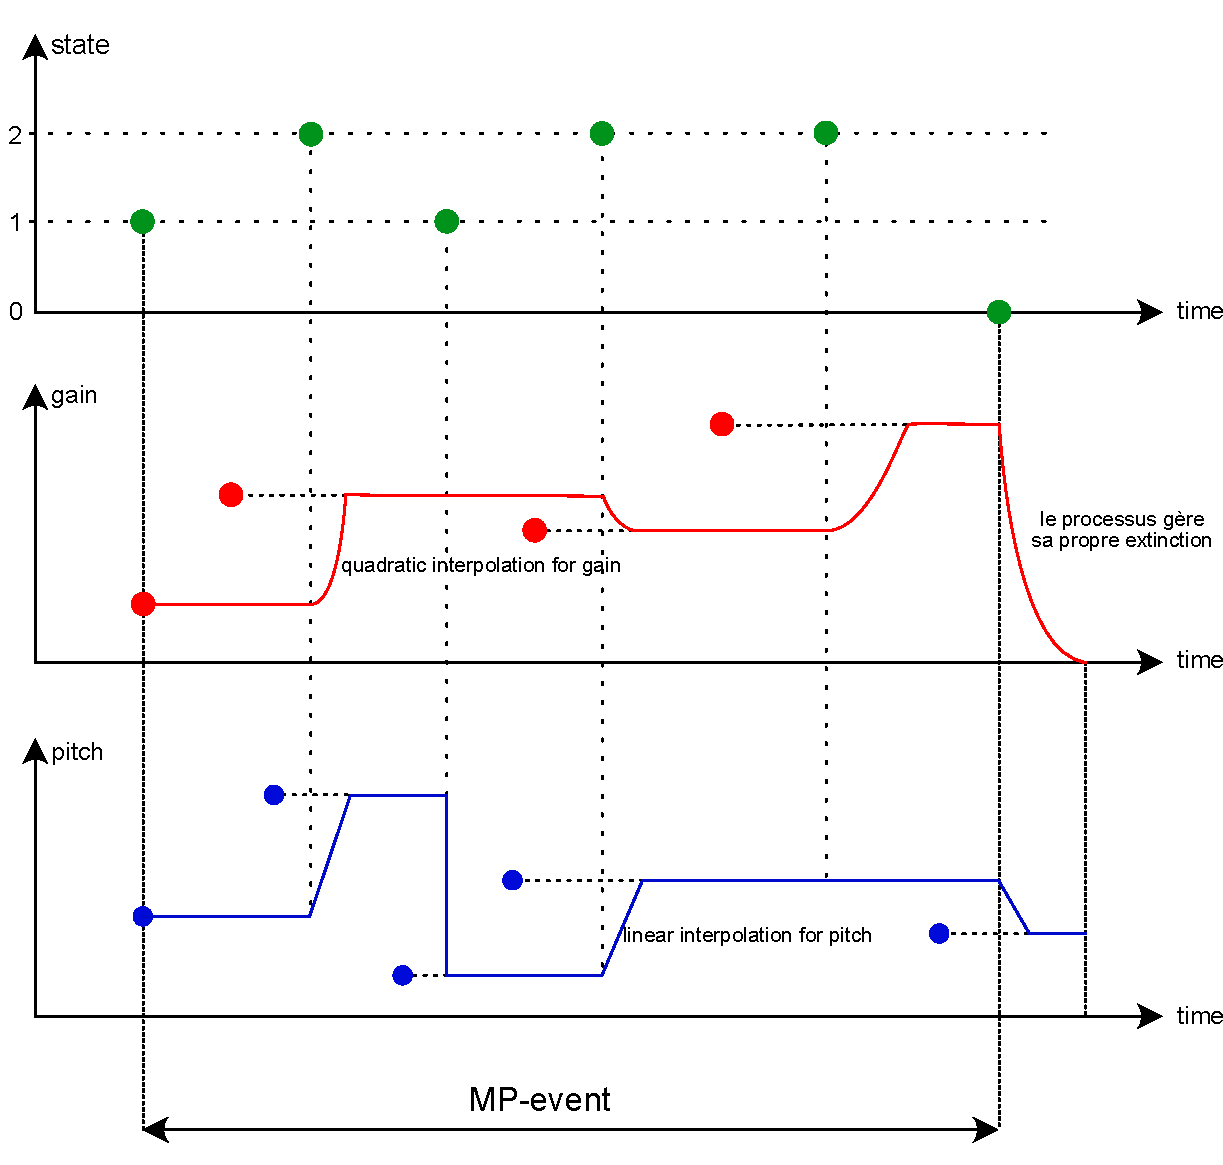
\includegraphics[width=\linewidth]{gfx/04_algorithms/MP-event-model.pdf}
%		\caption[Représentation schématique d'un \textit{MP-event}]{Représentation schématique d'un \%textit{MP-event}. Les cercles pleins représentent les états \textit{on}, les cercles vides les %états \textit{off} et les lignes continues les états \textit{update}.}
%		\label{fig:algorithms:MP-event-model}
%	\end{minipage}
%	\hspace{.02\linewidth}
%	\begin{minipage}[t]{0.48\textwidth}
%	  
\includegraphics[width=\linewidth]{gfx/dummy.pdf}
%		\caption[dummy]{dummy}
%		\label{fig:algorithms:dummy-1}
%	\end{minipage}
%\end{figure}
%------------------ Figure : MP-event et MP-block ---------------------

%------------------ Figure : MP-event ---------------------
\begin{figure}[!htbp]
	\captionsetup{format=plain}
	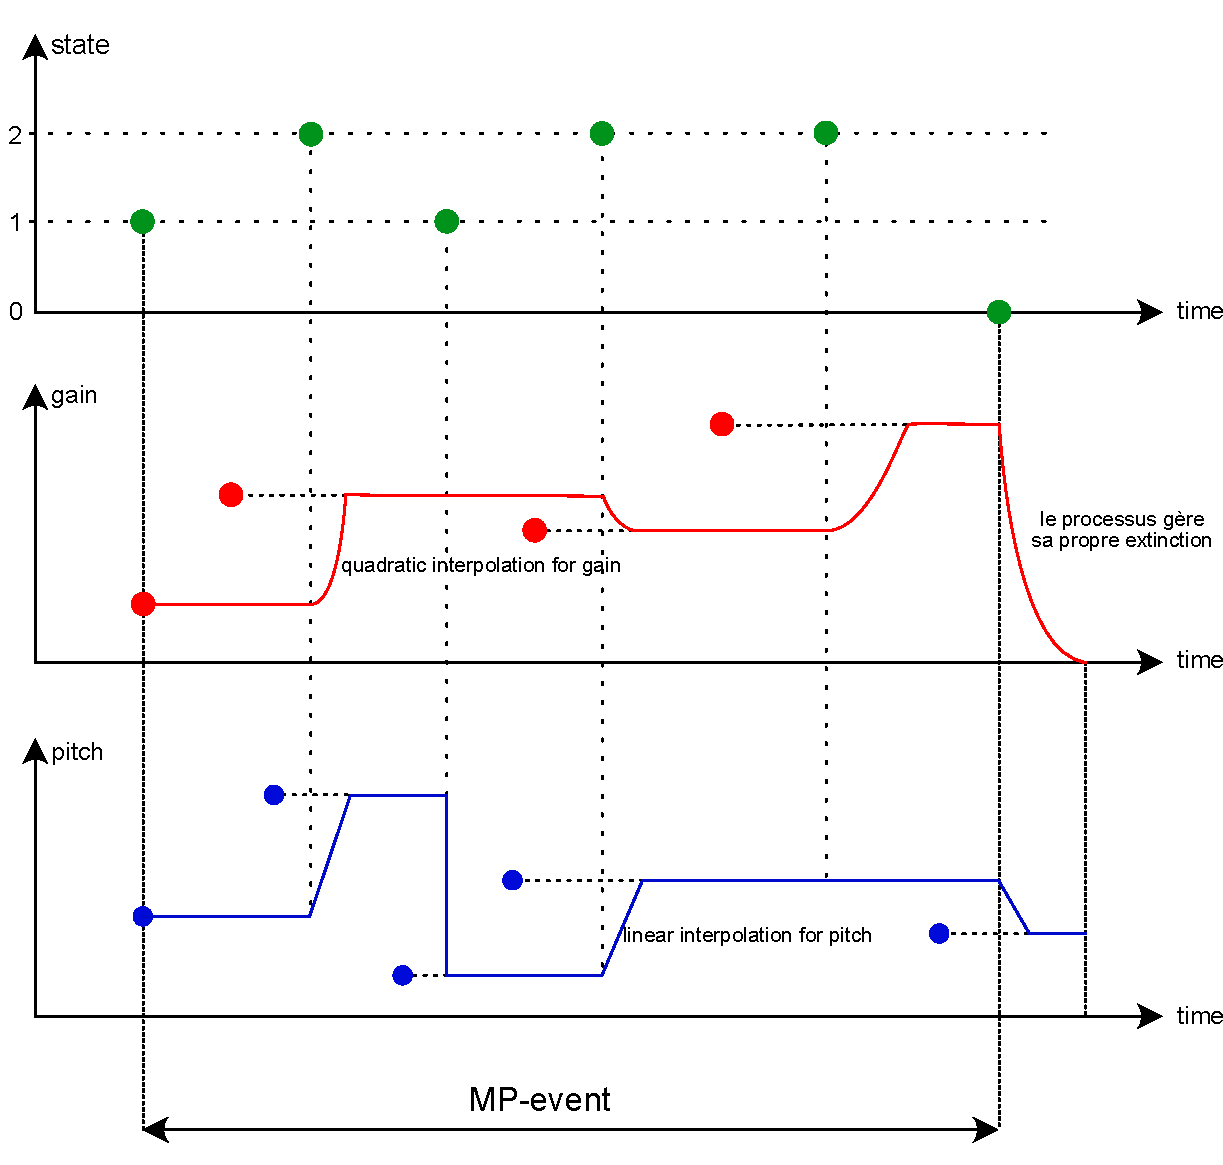
\includegraphics[width=\textwidth]{gfx/04_algorithms/MP-event-model.pdf}
	\caption[Représentation schématique d'un \textit{MP-event}]{Représentation schématique d'un \textit{MP-event}. Les cercles représentent des \textit{MP-messages}, les courbes représentent l'évolution du paramètre dans le processus. Noter que les paramètres ne sont pris en compte que lorsqu'un message \textit{state} est reçu.}
	\label{fig:algorithms:MP-event-model}
\end{figure}
%------------------ Figure : MP-event ---------------------


\subsubsection{Identifiant}

\noindent L'identifiant unique (ID) sert à identifier un \textit{MP-event} tout au long de ses traitements. Le \textit{MP-event} peut provenir d'un capteur physique (e.g. une touche de clavier) ou d'une source virtuelle (e.g. représentant le contact d'un doigt sur une \gls{TUI} ou le produit d'un algorithme génératif). L'ID est présent dans chaque \textit{MP-message} pour éviter toute erreur de routage dans le cas où un \textit{MP-block} reçoit parallèlement des \textit{MP-events} de plusieurs sources indépendantes. Les ID peuvent être définis explicitement --~auquel cas la gestion de conflit d'adressage est laissé à la charge du développeur~-- ou générés de manière unique par un objet dédié : \verb|mp.uID.maker|.

\subsubsection{Etat}

\noindent Le message ``\verb|state|'' est réservé et deux missions lui sont attribuées :
\vspace{-1em}
\begin{itemize}[noitemsep]
	\item il sert d'horloge asynchrone en déclenchant l'envoi des paramètres au processus;
	\item il spécifie la manière dont le processus doit interpréter ces paramètres.
\end{itemize}

\noindent Les paramètres peuvent ainsi être interprétés de trois façons :

\vspace{-1em}
\begin{itemize}[noitemsep]
	\item \textbf{state 1} : début de modulation de paramètre;
	\item \textbf{state 2} : mise à jour de paramètre;
	\item \textbf{state 0} : fin de modulation de paramètre.	
\end{itemize}

\noindent Le modèle musical sous-jacent envisage ainsi un \textit{MP-event} comme la modulation d'un ensemble de paramètres et prend en compte les phénomènes transitoires qui peuvent apparaître au début et/ou à la fin d'une modulation\footnote{ Un exemple évident est l'attaque d'un son, mais en ce qui concerne un processus non-sonore comme le filtrage de données, cela peut concerner l'initialisation du filtre.}. Ces discontinuités peuvent causer des réponses non-linéaires, trop rapides pour être contrôlées manuellement et parfois mieux traitées séparément.\\
\indent Dans l'algorithme de traitement, ces états peuvent correspondre à l'initialisation de variables internes, l'activation d'un lissage (\textit{portamento}) entre deux valeurs consécutives, le déclenchement d'un processus transitoire spécifique (e.g. l'attaque d'un son), etc. Tout paramètre peut donc être envoyé à un \textit{MP-block} en spécifiant s'il doit être considéré comme le début, la continuation ou la fin d'une phrase de modulation\footnote{ La confusion entre le \textit{pitch} et l'identifiant de note dans le protocole \gls{MIDI} rend le résultat de la même opération incertain : alors que certains synthétiseurs re-déclencheront la même voix, d'autres alloueront une nouvelle voix et attendront le même nombre de \textit{note-off} qu'il y a eu de \textit{note-on}.}. Ce modèle à trois états semble correspondre par ailleurs aux intentions de la \gls{MMA} qui a annoncé un message de \textit{note-update} dans le futur protocole MIDI-HD\footnote{Rapporté par le site web Synthopia: \url{http://www.synthtopia.com/content/2013/01/20/midi-manufacturers-testing-new-high-definition-midi-protocol/}}.\\
\indent Notons toutefois que dans notre cas, le message d'état peut être rattaché à n'importe quel paramètre, ce qui diffère encore de l'implémentation \gls{MIDI}, notamment en ce qui concerne l'allocation de voix. Alors que le premier message \verb|state 1| reçu pour un ID causera l'allocation d'une voix dans le \textit{MP-block}, le message \verb|state 0| ne libérera pas nécessairement cette voix, cette décision revenant au processus en cours, comme nous le verrons plus loin.

\subsubsection{Guest-list}

\noindent La spécification MP ne suit pas d'organisation hiérarchique telle que les canaux \gls{MIDI} ou les familles d'instruments de \gls{ZIPI}. À la place, elle laisse la possibilité à tout \textit{MP-event} de déclarer une liste de \textit{MP-events} ``invités'' (\textit{guestlist}) à la volée. Ces invités pourront avoir accès à la voix allouée au \textit{MP-event} hôte et contrôler ses paramètres. Cette fonctionnalité nous offre une solution flexible pour le groupement d'événements, permettant un nombre arbitraire de niveaux hiérarchiques, sans pour autant être limité par une relation de subsumption.\\
\indent La \textit{guestlist} peut être utilisée dans le cas de \textit{MP-blocks} génératifs, où l'ID du \textit{MP-event} ``parent'' peut être ajouté à la guestlist des \textit{MP-events} ``enfants''. Ceci permet une modulation cohérente de plusieurs voix associées à des \textit{MP-events} générés par une même source. Des exemples concrets de cette situation sont les pistes \gls{MIDI} ou la hiérarchie orchestre/famille/instrument/note proposée par \gls{ZIPI}. Ils correspondent à un ``\textit{\gls{mapping}} divergent'' dans le schéma proposé par Rovan, Wanderley, Dubnov et al. \cite{rovan_instrumental_1997}.\\
\indent Un ``\textit{\gls{mapping}} convergent'' est également possible : plusieurs \textit{MP-events} peuvent être déclarés comme invités d'un \textit{MP-event} tiers. Par exemple, un \textit{MP-event} ``enfant'' peut être créé à partir du résultat de l'interaction de plusieurs \textit{MP-events} ``parents'' (cf. exemple section \ref{sec:algorithms:many-guests-to-one}).\\
\indent Notons qu'une solution alternative aurait pu consister à transmettre systématiquement la liste de tous les paramètres d'un \textit{MP-event} parent à ses enfants. Dans le cas de chaînes de mapping assez longues, ou de polyphonies élevées, cet héritage systématique s'avérait cependant trop lourd pour être une solution efficace.


\subsubsection{Master-ID}

\noindent Le paramètre guests ne nous laisse toutefois pas un accès aisé à l'ensemble des voix de polyphonies d'un \textit{MP-block}. À cette fin, un identifiant spécifique indexé 0, permet ce contrôle global. Il revient implicitement à considérer que le \textit{MP-event} \#0 (nommé master-ID) fait systématiquement partie de la guestlist de tout \textit{MP-event}. Dans le cas où les \textit{MP-events}, ses \textit{guests} et le master-ID tentent de modifier les mêmes paramètres, l'ordre de priorité est donné du plus spécifique au plus général, c'est-à-dire, au \textit{MP-event}, puis aux \textit{guests}, puis au \textit{Master-ID}\footnote{On retrouve également cette idée, quoique limitée par les contraintes du \gls{MIDI}, dans la notion de \textit{master channel} du protocole \gls{MPE}.}.

\subsubsection{Ordonnancement des MP-messages}

\noindent Le cycle de vie de la voix d'un \textit{MP-event} suit la séquence suivante de \textit{MP-messages} :
\vspace{-1em}
\begin{enumerate}[noitemsep]
	\item envoi des paramètres de début de modulation;
	\item envoi du message state 1;
	\item envoi des paramètres de modulation;
	\item envoi du message state 2;
	\item envoi des paramètres de fin de modulation;
	\item envoi du message state 0.
\end{enumerate}
\noindent Cependant, comme la libération d'une voix ne suit pas nécessairement un message \verb|state 0| (dans le cas où le processus a sa propre stratégie d'extinction), il est possible d'envoyer différents messages d'état plusieurs fois durant la durée de vie d'une voix, jusqu'à ce que la voix soit effectivement libérée.

%-----------------------------------------------------------------------------------
\subsection{MP-blocks}

\noindent Un \textit{MP-block} se compose de deux parties (cf. schéma \ref{fig:algorithms:MP-block-model} et implémentation dans Max, figure \ref{fig:algorithms:MP-simpleSynth}) : le routeur et le traitement polyphonique que nous décrivons ici.

%------------------ Figure : MP-block ---------------------
\begin{figure}[!htbp]
	\captionsetup{format=plain}
	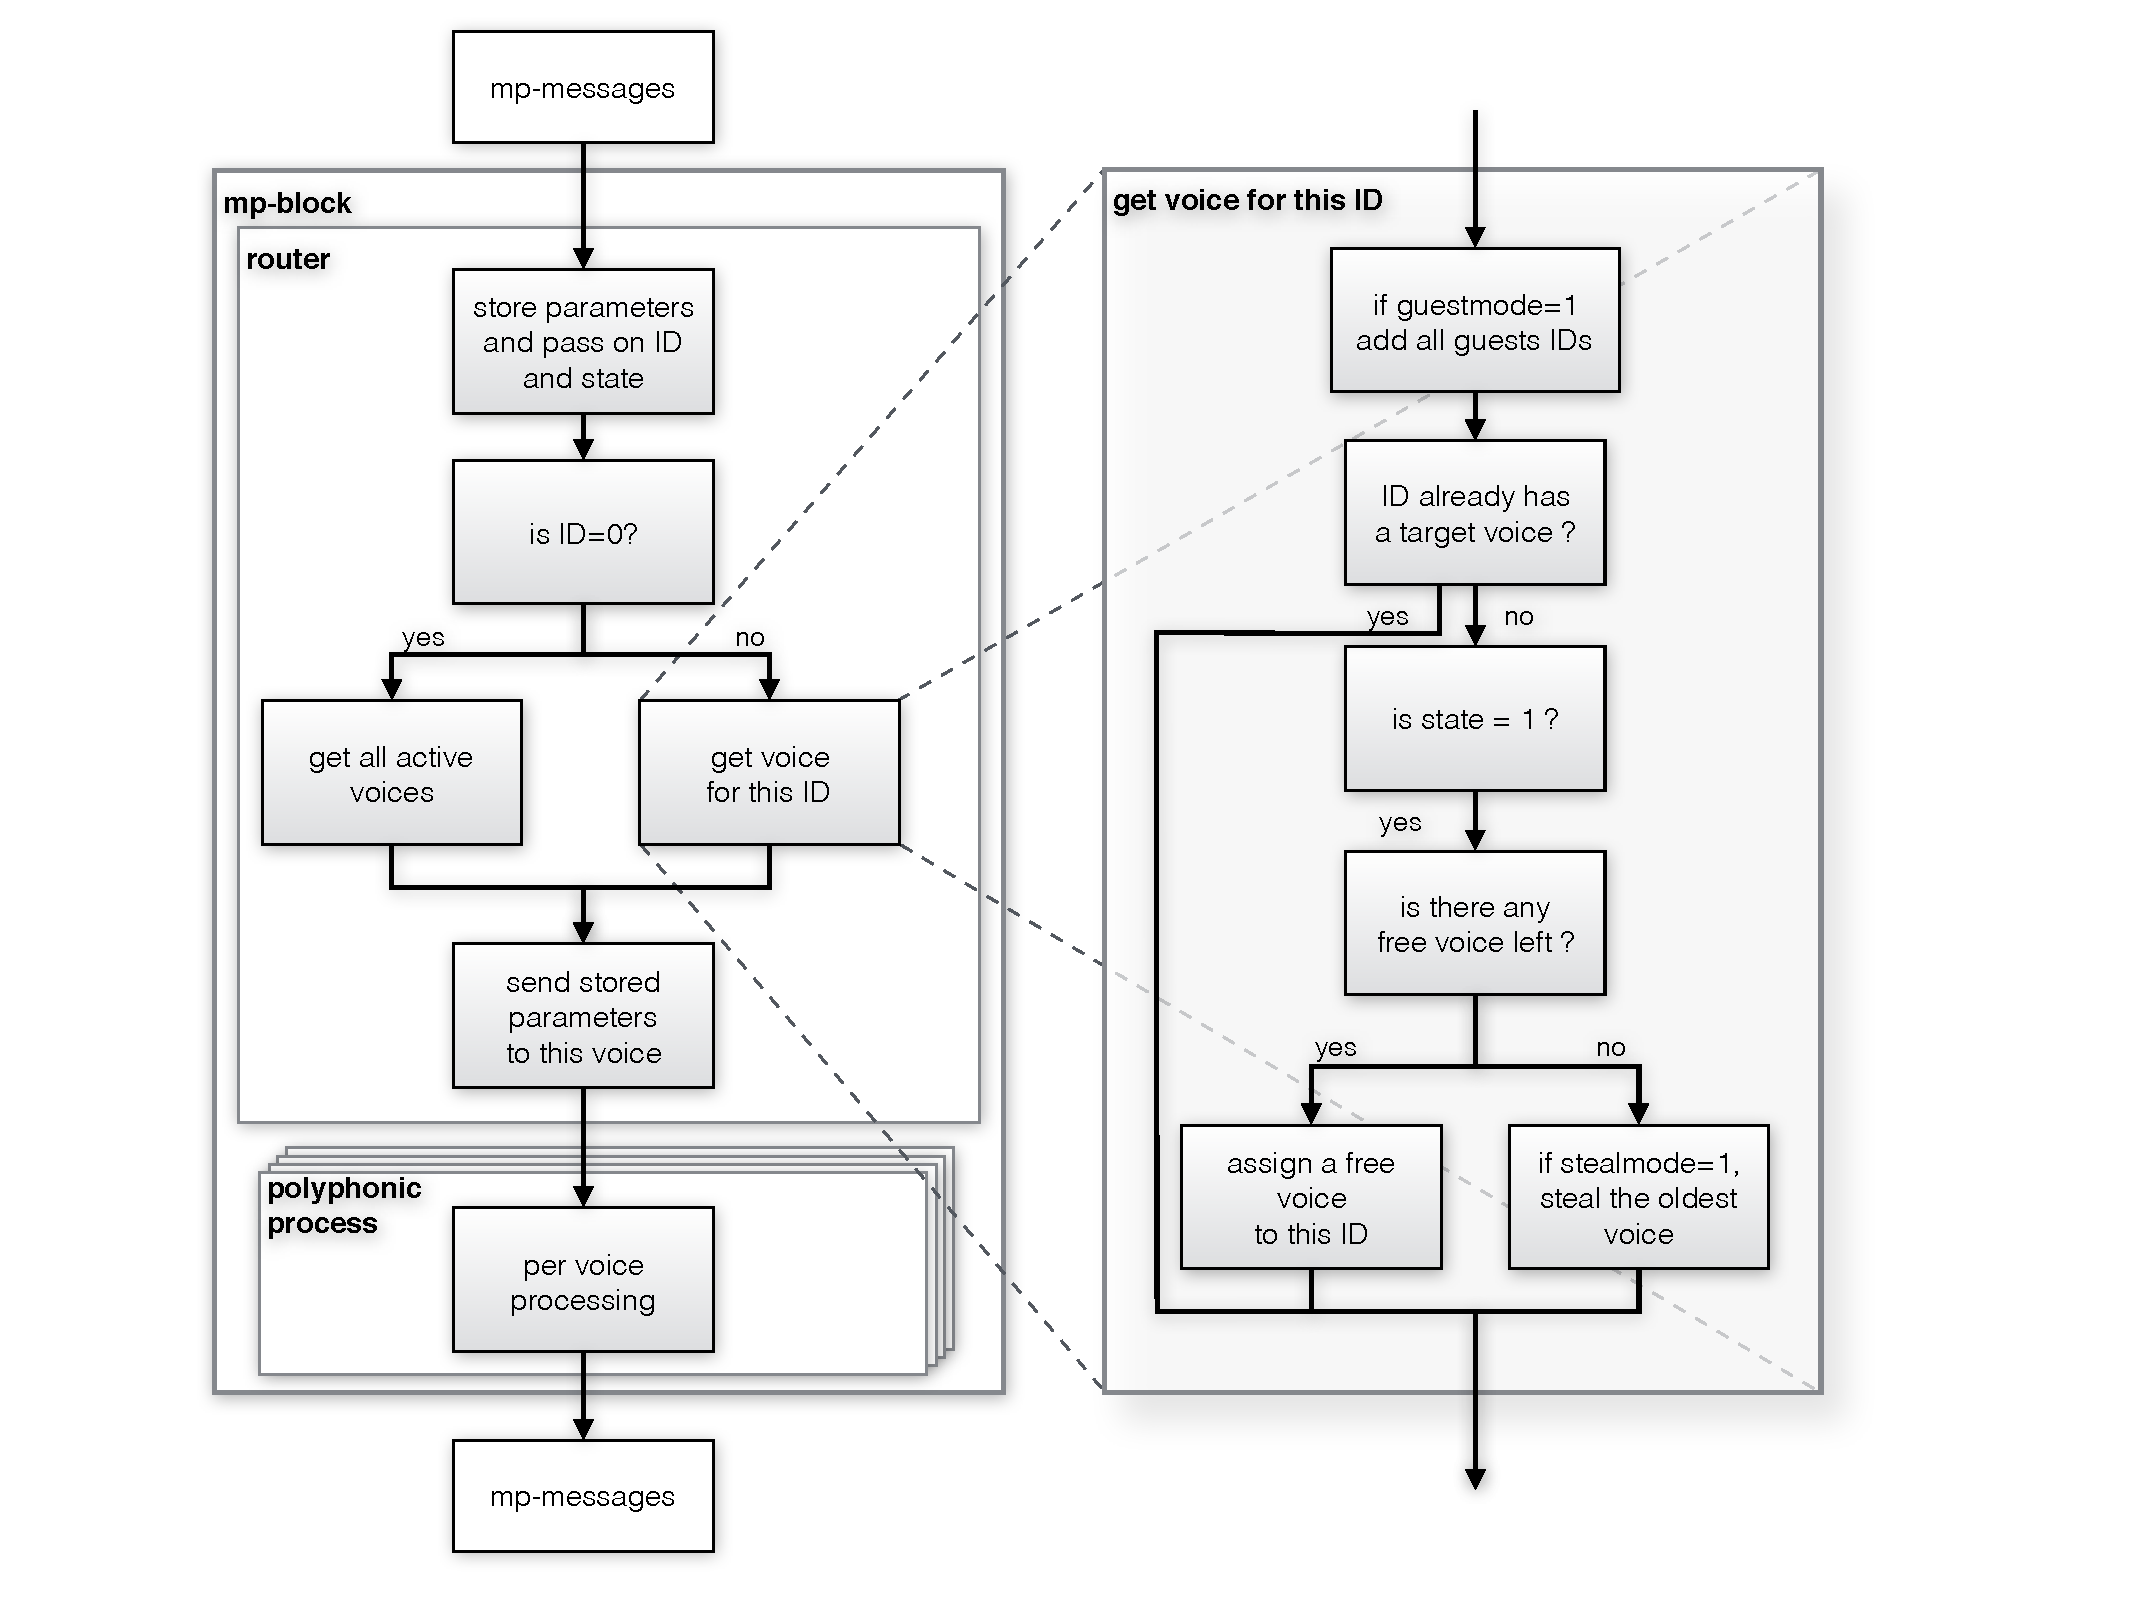
\includegraphics[width=\textwidth]{gfx/04_algorithms/MP-block-model.pdf}
	\caption[Représentation schématique d'un \textit{MP-block}]{Représentation schématique d'un \textit{MP-block} avec le fonctionnement du routeur.}
	\label{fig:algorithms:MP-block-model}
\end{figure}
%------------------ Figure : MP-block ---------------------


\subsubsection{Le routeur}

\noindent Le routeur accomplit les fonctions suivantes :
\vspace{-1em}
\begin{itemize}[noitemsep]
	\item le stockage des paramètres reçus pour un \textit{MP-event};
	\item l'allocation de voix pour un nouvel \textit{MP-event};
	\item l'envoi des paramètres à cette voix;
	\item l'envoi éventuel des paramètres des \textit{guests};
	\item d'enregistrer la libération de la voix.
\end{itemize}

\noindent L'ordonnancement des messages envoyés à la voix de traitement assure une synchronisation du calcul afin qu'il ne soit fait qu'une seule fois. Ainsi, la séquence suivante est envoyée par le routeur à la voix cible :
\vspace{-1em}
\begin{enumerate}[noitemsep]
	\item start X state Y : ce message permet à la voix de se préparer à traiter les paramètres à venir selon l'état Y;
	\item tous les paramètres du master-ID;
	\item tous les paramètres des guests;
	\item tous les paramètres du \textit{MP-event} déclencheur;
	\item end X state Y : ce dernier message clôt la séquence et sert de signal d'horloge déclenchant le calcul.
\end{enumerate}

\noindent L'allocation de voix est réalisée à l'arrivée du premier message \verb|state 1| pour un \textit{MP-event} donné. La libération de la voix intervient quand le processus de traitement indique au routeur qu'il a terminé sa tâche. Trois scénarios sont alors possibles :
\vspace{-1em}
\begin{itemize}[noitemsep]
	\item Le processus se termine dès qu'un message \verb|state 0| est reçu. Ce sera le cas, par exemple, pour un processus tel qu'une addition ou un filtre médian. Ce scénario est pris en compte de manière automatique en spécifiant un attribut \verb|@automute 1| au routeur;
	\item Le processus déclenche son extinction à la réception d'un message \verb|state 0|, typiquement le release d'une enveloppe \gls{ADSR};
	\item Le processus a sa propre durée et peut avoir terminé sa tâche avant ou après avoir reçu un message state 0. C'est le cas, par exemple, lors de la génération d'un signal audio de durée fixe comme un échantillon de percussion.
\end{itemize}

\subsubsection{Traitement par voix}

\noindent Le traitement par voix est effectué par un patch chargé dans les multiples voix d'un objet Max \verb|poly~|. En dehors des fonctions permettant le traitement à proprement parler, un objet nommé \verb|mp-muter| permet de ventiler les messages envoyés par le routeur en fonction du message d'état et de renvoyer au routeur l'information de fin de tâche que le processus doit fournir dans le cas où il possède une extinction propre (mode \verb|@automute 0|). Ce principe est exposé sur la figure \ref{fig:algorithms:MP-simpleSynth-inside}, dans laquelle l'objet Max \verb|adsr~| vient notifier la fin de l'enveloppe à l'objet \textit{mp.muter}.

%------------------ Figure : simple synth ---------------------
\begin{figure}[!htbp]
	\captionsetup{format=plain}%
	\centering
	\begin{minipage}[t]{0.510\textwidth}
		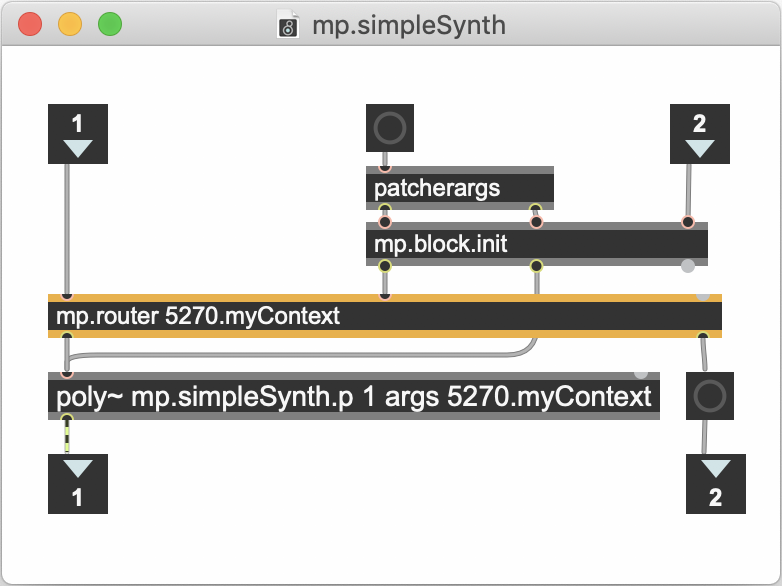
\includegraphics[width=\linewidth]{gfx/04_algorithms/MP-reallySimpleSynth.png}
		\caption[mp.simpleSynth : encapsulation de la synthèse]{mp.simpleSynth : routeur et encapsulation de la synthèse.}
		\label{fig:algorithms:MP-simpleSynth}
	\end{minipage}
	\hspace{.02\linewidth}
	\begin{minipage}[t]{0.450\textwidth}
	  	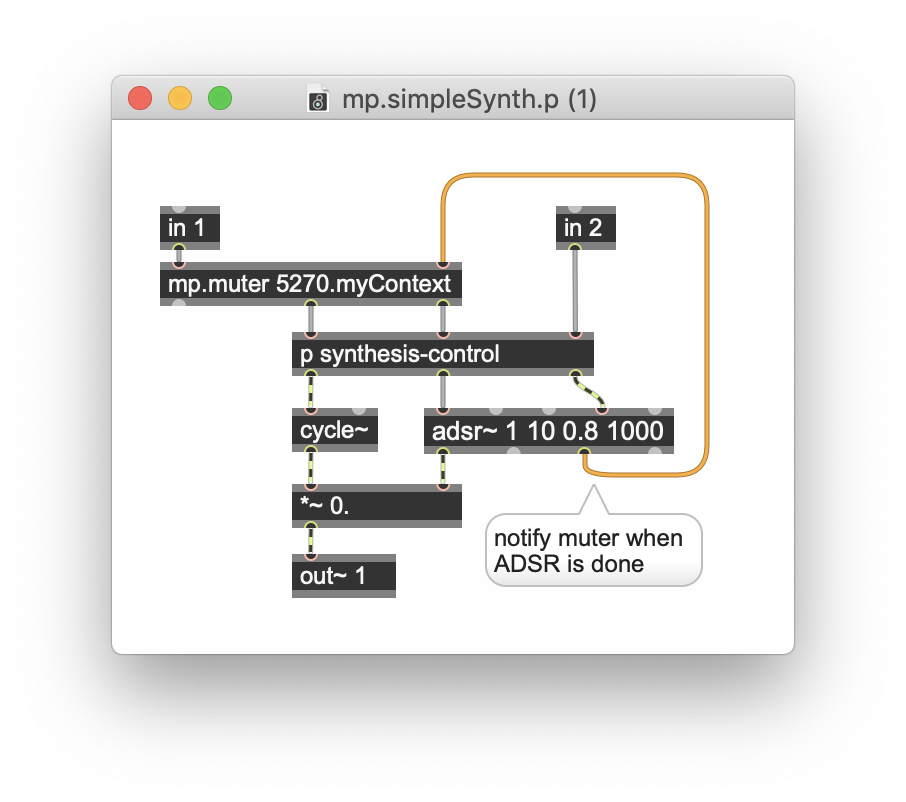
\includegraphics[width=\linewidth]{gfx/04_algorithms/MP-reallySimpleSynth-inside.png}
		\caption[mp.simpleSynth : patcher de synthèse]{mp.simpleSynth : patcher de synthèse. Le routeur est notifié de la fin d'activité de l'envoi d'un message ``mute'' par l'objet ADSR.}
		\label{fig:algorithms:MP-simpleSynth-inside}
	\end{minipage}
\end{figure}
%------------------ Figure : simple synth ---------------------


\subsubsection{Paramètres d'un MP-block}

\noindent Les \textit{MP-blocks} répondent à une liste de paramètres contrôlant le processus de traitement par voix. Ces paramètres sont stockés par ID dans le routeur jusqu'à ce qu'un message d'état soit reçu. Ce message entrainera l'allocation d'une voix (si disponible), à qui seront envoyés tous les paramètres rattachés à cet ID.\\
\indent Il est possible d'envoyer d'autres paramètres que ceux contrôlant le processus. Dans ce cas il traverseront le \textit{MP-block} inchangés, tout en restant synchrones avec d'éventuels autres paramètres générés par le processus qu'ils traversent. Dans le cas où ce processus génère de nouveaux \textit{MP-events}, ces paramètres peuvent automatiquement être ajoutés à chaque \textit{MP-event} généré, en une sorte d'héritage similaire à celui opéré par la librairie ``o.'' \cite{freed_composability_2011}, mais non-automatique et laissé à l'appréciation du développeur du \textit{MP-block}.

%-----------------------------------------------------------------------------------
\subsection{Exemples}

\noindent Les exemples proposés dans cette section présentent des cas concrets d'utilisation du système MP. Ils sont implémentés dans le logiciel Max et inclus dans les exemples du package \textit{ModularPolyphony}. Ces exemples s'appuient sur l'utilisation d'une tablette \textit{multitouch}, dont les données reçues dans l'objet \verb|mp.TUIO.input| sous la forme de \textit{MP-events} correspondent au contact de chaque doigt, avec les coordonnées en X et Y de leur position sur la tablette. Le synthétiseur \verb|mp.simpleSynth| est celui présenté sur les figures \ref{fig:algorithms:MP-simpleSynth} et \ref{fig:algorithms:MP-simpleSynth-inside}.

\subsubsection{Mapping simple avec une fonction pure}

\noindent Cet exemple (figure \ref{fig:algorithms:MP-pure}) montre l'utilisation la plus simple du système MP. On contrôle ici la valeur de vélocité sur l'axe vertical tandis que l'axe horizontal contrôle la hauteur.\\
\indent Comme l'objet \verb|scale|, qui opère une mise à l'échelle entre les données de position (entre 0 et 1) et les données de hauteur et de vélocité (en valeur \gls{MIDI} 0-127), est une fonction pure\footnote{En informatique, une fonction pure, appelée également algortihme déterministe, est une fonction dont la sortie ne dépend que de la valeur d'entrée.}, il peut être utilisé pour traiter directement l'ensemble des \textit{MP-messages} lui parvenant. Ici, l'avantage d'utiliser MP est de bénéficier d'un système d'adressage similaire au \gls{MPE} sans être limité par le typage, la précision et l'espace de nommage des données.

%------------------ Figure : simple synth ---------------------
\begin{figure}[!htbp]
	\captionsetup{format=plain}%
	\centering
	\begin{minipage}[t]{0.485\textwidth}
		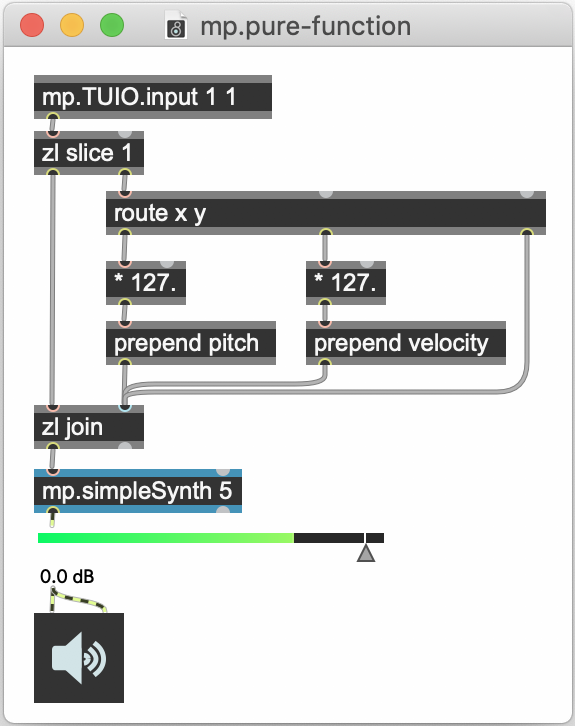
\includegraphics[width=\linewidth]{gfx/04_algorithms/MP-mappingPure.png}
		\caption[Exemple de patch MP : fonction pure]{Exemple de patch MP : mapping avec une fonction pure.}
		\label{fig:algorithms:MP-pure}
	\end{minipage}
	\hspace{.01\linewidth}
	\begin{minipage}[t]{0.485\textwidth}
	  	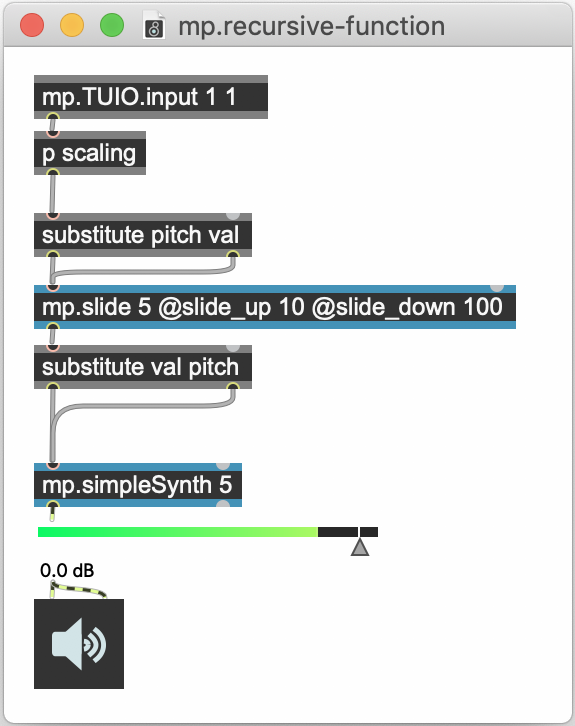
\includegraphics[width=\linewidth]{gfx/04_algorithms/MP-mappingRecursive.png}
		\caption[Exemple de patch MP : fonction récursive]{Exemple de patch MP : mapping avec une fonction récursive.}
		\label{fig:algorithms:MP-recursive}
	\end{minipage}
\end{figure}
%------------------ Figure : simple synth ---------------------

\subsubsection{Mapping avec une fonction impure}

\noindent Une fonction sera impure dans le cas où son fonctionnement interne implique la mémorisation de valeurs. Ce cas de figure se produit avec les fonctions récursives, mais également avec les fonctions non-récursives, quand leurs différents opérandes arrivent de manière non-synchrone.\\
\indent Cet exemple (figure \ref{fig:algorithms:MP-recursive}) montre le cas d'un mapping avec une fonction récursive. L'objet \verb|slide| de Max opère un filtrage logarithmique définit par l'équation :
 $$y[n] = y[n-1] + \frac{(x[n]-y[n-1])}{slide}$$ 
\noindent Dans ce cas là, il n'est plus possible d'utiliser une seule instance de l'objet \verb|slide| pour traiter l'ensemble des \textit{MP-messages}, en raison de la mémoire interne d'un état précédant propre à un \textit{MP-event} particulier. L'objet \verb|mp.slide| permet alors d'instancier plusieurs voix traitant les valeurs individuelles de \textit{pitch} en parallèle.


\subsubsection{Création dynamique de MP-events et guests}

\noindent Dans cet exemple (figure \ref{fig:algorithms:MP-mappingDivergent}), nous créons à la volée des \textit{MP-events} ``enfants'' que nous contrôlons en parallèle avec le \textit{MP-event} ``parent''.
Dans un premier temps, nous associons les coordonnées x et y d'un \textit{MP-event} aux paramètres de hauteur (pitch) et de vélocité, respectivement. Le module \verb|mp.note2chord| génère un accord à partir de la hauteur (ici en ajoutant une quinte à la hauteur d'entrée). Cet accord prend la forme de deux nouveaux \textit{MP-events} enfants qui vont venir activer chacun une voix de polyphonie de notre synthétiseur. Le module \verb|mp.note2chord| ajoute également aux paramètres des \textit{MP-events} enfants, l'ID du \textit{MP-event} parent, en tant qu'invité. Ceci va nous permettre de contrôler le paramètre de vélocité des deux notes simultanément à partir du \textit{MP-event} parent. 

\vspace{-1em}
\begin{itemize}[noitemsep]
	\item à gauche, le module  génère un ensemble de \textit{MP-events} "enfants". Le premier niveau en génère deux et le deuxième niveau en génère 3. Le résultat final est la génération d'un accord de six notes à partir d'un seul \textit{MP-event};
	\item à droite, le \textit{MP-event} venant de \textit{mp.TUIO.input} est envoyé sur deux chemins où ses valeurs sont mises à l'échelle par le module mp-scale pour définir la fréquence et l'offset d'un LFO respectivement. Le \gls{LFO} contrôlera ensuite la fréquence de coupure d'un filtre passe-bas du module de synthèse;
	\item nous avons deux occurrences d'un contrôle global avec le Master-ID : une pour le paramètre \textit{depth} du LFO et une pour la transposition du deuxième étage \textit{note2chord};
	\item en dernier lieu, nous dirigeons les messages résultants de ces deux chemins vers un système de représentation graphique. La position d'objets graphiques est assignée aux valeurs de pitch des \textit{MP-events} générés, tandis que leur couleur est associée au \textit{MP-event} parent. Ceci résulte en une représentation graphique de toutes les hauteurs en tant qu'objets dont la couleur nous dit à quelle source commune (ici le contact d'un doigt sur un écran) ils sont rattachés.
\end{itemize}

%------------------ Figure : simple synth ---------------------
\begin{figure}[!htbp]
	\captionsetup{format=plain}%
	\centering
	\begin{minipage}[t]{0.38\textwidth}
		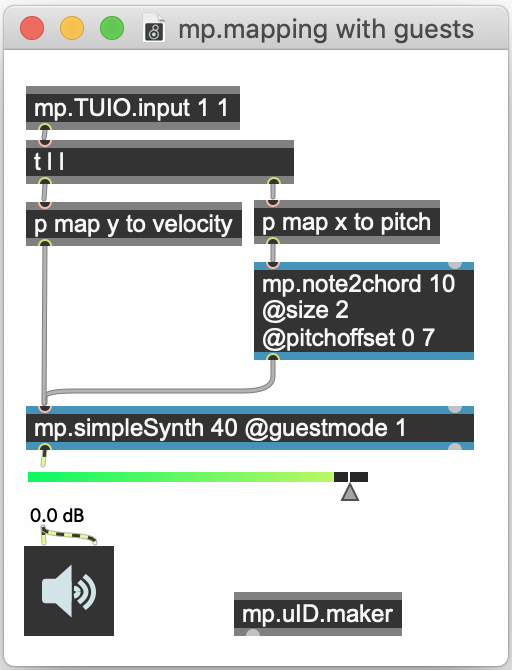
\includegraphics[width=\linewidth]{gfx/04_algorithms/MP-mappingGuest.png}
		\caption[Exemple de patch MP : guestlist]{Utilisation de la guestlist pour un mapping divergent.}
		\label{fig:algorithms:MP-mappingDivergent}
	\end{minipage}
	\hspace{.01\linewidth}
	\begin{minipage}[t]{0.58\textwidth}
	  	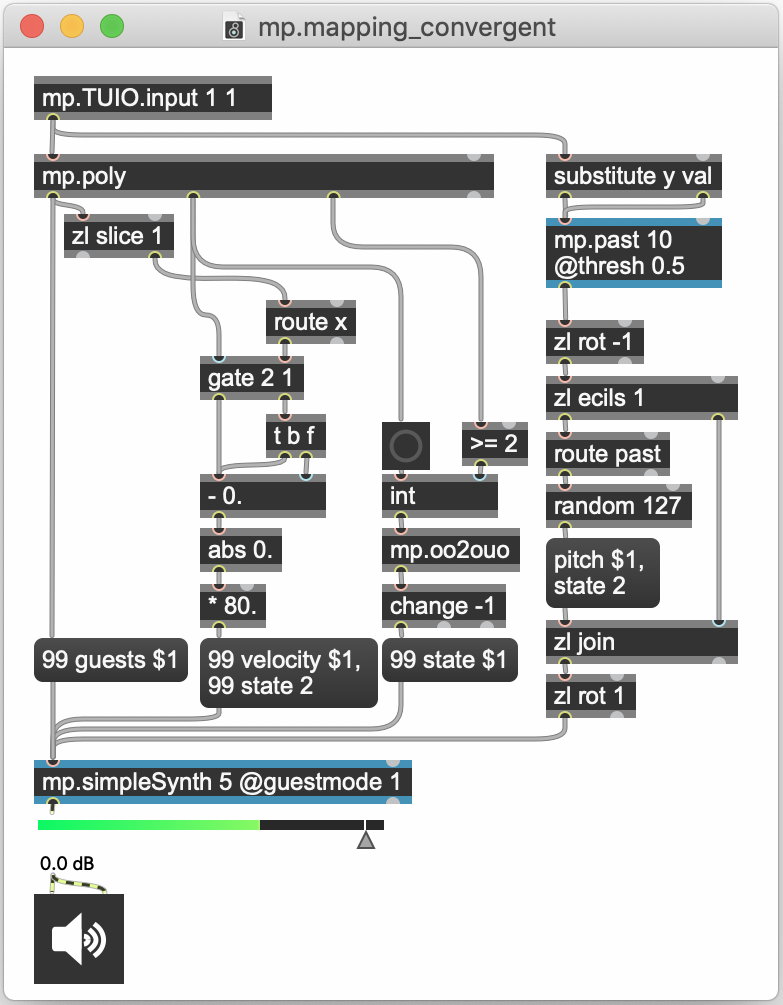
\includegraphics[width=\linewidth]{gfx/04_algorithms/MP-mappingConvergent.png}
		\caption[Exemple de patch MP : guestlist]{Utilisation de la guestlist pour un mapping convergent.}
		\label{fig:algorithms:MP-convergent}
	\end{minipage}
\end{figure}
%------------------ Figure : simple synth ---------------------


\subsubsection*{Mapping polyphonique convergent: many[guests]-to-one}
\label{sec:algorithms:many-guests-to-one}

\noindent Alors que l'exemple précédant montre une utilisation de la \textit{guestlist} dans un mapping ``divergent'', le suivant (figure \ref{fig:algorithms:MP-convergent}) réalise un mapping ``convergent''.\\
\indent Imaginons que l'on souhaite contrôler avec deux doigts un son dont l'intensité est proportionnelle à l'espacement de nos doigts. Il faut alors que deux \textit{MP-events} indépendants (correspondants à la captation de mes deux doigts) soient combinés pour que leur présence conjointe donne naissance à un nouveau \textit{MP-event} ``enfant''. C'est ce qui est réalisé dans les deux chaînes de traitement centrales sur la figure \ref{fig:algorithms:MP-convergent}, la chaîne la plus à gauche déclarant les ID des \textit{MP-events} ``parents'' dans la \textit{guestlist} du MP-event ainsi créé.\\
\indent Imaginons maintenant que l'on souhaite que la hauteur du son produit change aléatoirement à chaque fois que l'un de nos doigts franchit une frontière virtuelle sur l'interface (définie dans l'exemple de la fiure \ref{fig:algorithms:MP-convergent} comme une ligne horizontale de coordonnée $y=0,5$). Cela nécessite que les \textit{MP-events} correspondant à chacun de mes doigts puissent agir sur le son créé par le \textit{MP-event} ``enfant''. C'est l'opération réalisée par la chaîne de traitement la plus à droite sur la figure \ref{fig:algorithms:MP-convergent}, avec l'objet \verb|mp.past| qui détecte le franchissement de seuil pour chaque événement en parallèle (cette détection n'étant pas une fonction pure).


\subsubsection*{Contrôle d'interfaces graphiques}
\label{sec:algorithms:example-mpTUI}
\noindent Le système MP est également amplement utilisé dans la librairie MP.TUI, détaillée au chapitre suivant.


\subsection{Limitations et optimisations}

\noindent Séparer les différents processus de traitement d'un design d'interaction polyphonique a l'avantage de permettre une meilleure modularité et, par suite, une meilleure stabilité des processus mis en œuvre, qui n'auront pas à être modifiés en interne pour être adaptés à une autre situation. Le choix a également été fait de ne pas s'appuyer sur une mémoire globale ou des pointeurs externes aux modules (e.g. pour sauver la guestlist), de sorte que les \textit{MP-blocks} sont réellement indépendants et autonomes et que le design d'interaction général puisse être réparti sur plusieurs applications et/ou machines en réseau.\\
\indent Cependant, cette modularité a un coût et est moins optimisée, en terme de computer et d'utilisation de la mémoire, qu'un design qui consisterait à inclure toutes les fonctions nécessaires dans les traitements \textit{ad-hoc}. Certaines optimisations peuvent être réalisées pour des processus ne nécessitant pas de mémoire interne (e.g. une mise à l'échelle statique), pour lesquels il n'est pas nécessaire d'allouer des voix. Cela se fait cependant au prix de certaines fonctionnalités (pas d'utilisation du \textit{master-ID} possible dans ce cas). Par ailleurs, le framework MP a entièrement été réalisé à l'aide d'objets natifs Max et pourrait sûrement être optimisé en le portant sous la forme d'objets compilés.\\
\indent Le modèle de messages asynchrones distinguant début et fin d'événement ne résoud pas directement le problème de note ``bloquées''\footnote{Ce problème surgit dans les systèmes MIDI, quand un message \textit{note-off} n'arrive pas au synthétiseur et que le son reste ainsi ``bloqué''. On trouve généralement sur les systèmes MIDI une fonction ``MIDI-panic'' qui règle brutalement ce problème en envoyant des messages \textit{note-off} sur toutes les voix.} tel qu'on le connait avec l'utilisation du \gls{MIDI}. Cependant, l'ouverture de l'espace de nommage permet l'implémentation \textit{ad-hoc} d'un système d'acquittement\footnote{tel qu'il existe dans le protocole \gls{TCP}}, ou de \textit{heartbeat}\footnote{Nom donné au signal périodique généré par un programme pour indiquer son fonctionnement normal ou pour sa synchronisation avec d'autres parties d'un système informatique.}. Également un message \textit{flush}\footnote{Equivalent de la fonction ``MIDI-panic'' généralement présente sur les système MIDI et permettant d'éteindre toutes les notes actives (quand elles sont bloquées).} est présent sur chaque module MP afin de gérer au besoin l'urgence lors d'une performance.


%%%%%%%%%%%%%%%%%%%%%%%%%%%%%%%%%%%%%%%%%
\section{Sagrada : extension de MP au DSP}
\label{sec:algorithms:sagrada}

%--------------------------------------------------------------------------------
\subsection{Motivations et contexte}

\noindent Si le développement de la librairie MP a permi d'apporter du contrôle continu à l'intérieur d'une logique basée sur des événements discrets, la démarche inverse permet d'explorer, dans l'autre sens, les passerelles expressives possibles entre le synchrone et l'asynchrone, entre le continu et le discret, le lisse et le strié\footnote{Pierre Boulez utilise ces termes pour évoquer la dialectique entre le continu et le discontinu et définir la nature des ``espaces'' (dont le temps, en particulier) en musique dans \cite{boulez_penser_1987}.}. En particulier, la synthèse granulaire est basée sur le découpage du continuum sonore en grains de son et les premières œuvres utilisant ce type de synthèse\footnote{Par exemple, ``ConcretPH'' de Iannis Xénakis en 1958, ou ``Kontakte'' de Karlheinz Stockhausen en 1960, dont un passage durant lequel la fréquence des grains, d'abord perçue comme une hauteur tonale, décroit jusqu'à être perçue comme un rythme, est un exemple concret notre propos.} sont très nettement marquée par cette recherche de passage entre le continu et le discret.\\
\indent Ma pratique personnelle m'avait amené à utiliser l'environnement GMU\footnote{Environnement pour la synthèse granulaire dans Max/MSP, développé par Laurent Pottier et Charles Bascou au \gls{GMEM}, voir \cite{bascou_gmu_2005}} en raison des possibilités inégalées qu'il offrait dans Max, en terme de contrôle du déclenchement des grains, réalisé par un signal \gls{DSP}, ce qui permet des fréquences de grains très élevées (potentiellement, jusqu'à la moitié de la fréquence d'échantillonage) tout en conservant une précision temporelle à l'échantillon près.\\
\indent La question était donc : comment relier ces deux domaines polyphoniques s'appuyant sur des supports hétérogènes ? La possibilité de pouvoir contrôler les grains individuellement dans GMU, bien que très fine, ne permettait pas d'accéder à leur modulation en dehors de l'interface fournie par l'objet Max. Les grains y sortent mixés sur deux canaux\footnote{Une version 8-canaux existe aussi, mais destinée plutôt pour l'octophonie de haut-parleurs, plutôt que pour le traitement individuel des grains.} et l'ajout d'un filtre en aval est nécessairement appliqué à l'ensemble des grains.\\
\indent Suivant la même logique de modularisation suivie dans le développement de MP, Sagrada propose un ensemble de modules indépendants, traitant les grains de manière indépendante. Le passage de paramètre est réalisé à partir d'une horloge qui envoit des impulsions sur un signal synchrone de Max.

%--------------------------------------------------------------------------------
\subsection{Implémentation}

\subsubsection{Types de modules}
\noindent Sagrada est basé sur trois types de modules, dont le fonctionnement est détaillé par la suite :
\vspace{-1em}
\begin{itemize}[noitemsep]
	\item \textbf{une horloge}, gérant le déclenchement des grains;
	\item \textbf{des modules de traitement}, contrôlés par l'horloge;
	\item \textbf{des modules de gestion de flux}, permettant de grouper les ticks d'horloges en flux indépendants.
\end{itemize}


\subsubsection{Interconnexion des modules}

\noindent Un patch Sagrada (figure \ref{fig:algorithms:MP-ExamplePatch}) fait intervernir une série de modules reliés par une variable définissant un \textit{contexte}. Ce contexte permet de :
\vspace{-1em}
\begin{itemize}[noitemsep]
	\item \textbf{redéfinir la polyphonie} de l'ensemble des modules, en la déclarant seulement auprès de l'horloge ;
	\item \textbf{synchroniser} l'ensemble des modules à une horloge commune;
	\item \textbf{éviter les conflit d'adressage} entre plusieurs contextes Sagrada.
\end{itemize}

\noindent Les modules de Sagrada sont interconnectés par la spécification du nom de leurs entrées et sorties sous forme d'arguments du module (à l'instanciation), ou de messages Max pour changer cette interconnexion à la volée.

%------------------ Figure : Sagrada-trigger ---------------------
\begin{figure}[!htbp]
	\captionsetup{format=plain}
	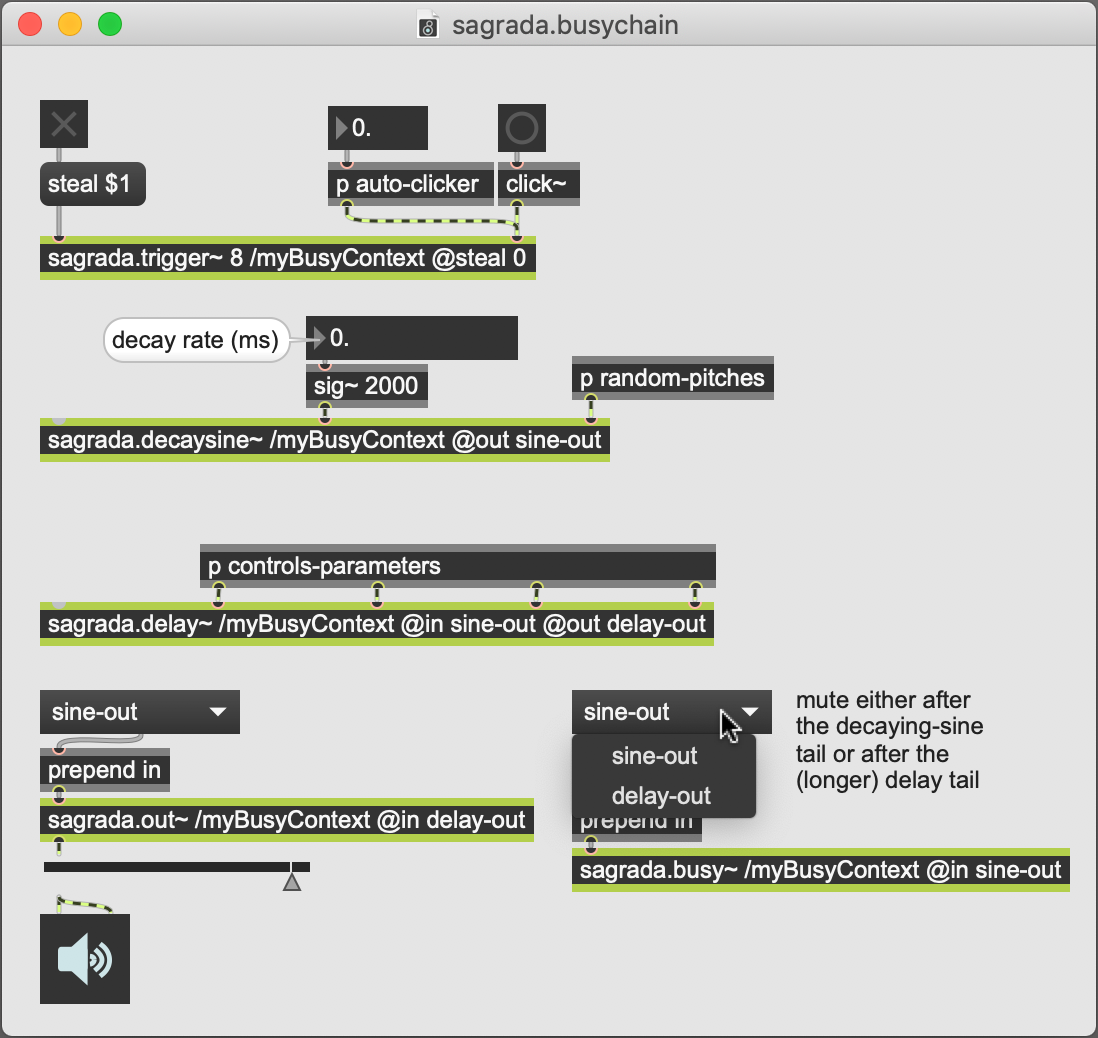
\includegraphics[width=\textwidth]{gfx/04_algorithms/Sagrada-examplePatch.png}
	\caption[Sagrada : exemple de patch]{Example de patch Sagrada montrant différents modules interconnectés dans un même contexte}
	\label{fig:algorithms:MP-ExamplePatch}
\end{figure}
%------------------ Figure : Sagrada-trigger ---------------------

\subsubsection{Horloge et assignation de voix}

\noindent L'horloge de Sagrada est implémentée dans l'abstraction Max \verb|sagrada.trigger~|. Son principe de fonctionnement consiste à envoyer un \textit{tick} de déclenchement de grain à une nouvelle voix de polyphonie à chaque fois qu'elle reçoit une impulsion en entrée. Ces impulsions peuvent donc être déclenchées soit de manière asynchrone (e.g. en transformant un message \gls{MIDI} en une une impulsion grâce à l'objet Max \verb|click~|), soit de manière synchrone (e.g. en utilisant un train d'impulsion controlé en fréquence). L'incrément fonctionne selon l'équation suivante, dans laquelle $x$ représente le signal de délenchement, $y$ la voix de polyphonie cible et $N$ la polyphonie maximale autorisée :
$$ y[n] = \big(x[n] + y[n - 1]\big) \mod N $$
\noindent Dans cette version simple, l'assignation des voix se fait donc de manière cyclique, en ``usurpant'' au besoin la voix à un grain encore actif. Un mécanisme de non-usurpation est également proposé sur le mode du \textit{round-robin}\footnote{Le \textit{round-robin} est un algorithme d'ordonnancement consistant à attribuer une opération à un processus faisant partie d'une file d'attente, en choisissant le premier disponible dans l'ordre de la file d'attente.}. Il s'appuie sur l'utilisation d'un tableau, nommé ``\textit{jump-buffer}'', contenant l'incrément nécessaire pour passer de la voix prévue par l'algorithme simple à la prochaine voix disponible. Si la voix prévue est libre, cet incrément est nul; si l'incrément est égal à la valeur de polyphonie, on n'envoit pas le grain, sinon on saute de offset du \textit{jump-buffer }pour trouver une voix libre.
$$ z[n] = \Big(y[n] + jump\big[y[n]\big]\Big)\mod N $$
\noindent L'implémentation de ce mécanisme d'horlge synchrone a été réalisé dans l'environnement \verb|gen~| de Max, afin de pouvoir travailler à l'échantillon (cf. figure \ref{fig:algorithms:Sagrada-TriggerClock}). Le calcul des valeurs du \textit{jump-buffer} est réalisé en permanence de manière synchrone (cf schéma fonctionnel figure) à partir de l'information d'état actif des voix, typiquement calculée à partir d'un seuillage sur l'enveloppe temporelle du son.\\
\indent Le module permettant ce mode de fonctionnement sans usurpation de voix est implémenté dans un module indépendant, pouvant être placé à n'importe quel endroit dans la chaîne de traitement des grains. (cf. objet \verb|sagrada.busy~| sur la figure \ref{fig:algorithms:MP-ExamplePatch}) Par exemple, si un grain subit une opération de filtrage résonnant, sa durée finale sera plus longue que le grain original. On pourra donc, au besoin, contrôler l'état occupé d'une voix par les grains issus de ce filtre résonnant.

%------------------ Figure : Sagrada-trigger ---------------------
\begin{figure}[!htbp]
	\captionsetup{format=plain}
	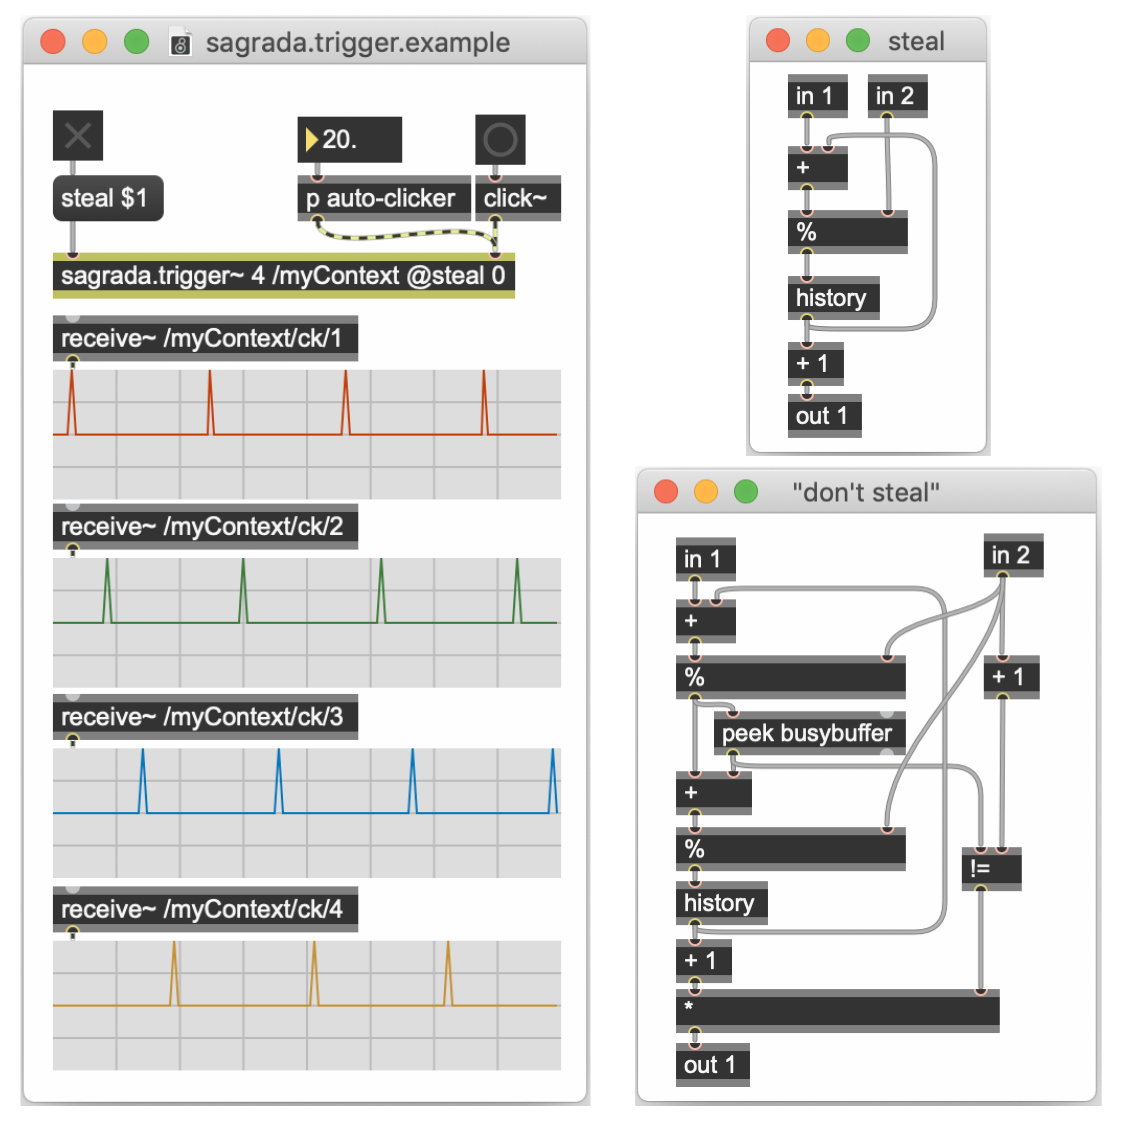
\includegraphics[width=\textwidth]{gfx/04_algorithms/Sagrada-TriggerClock.png}
	\caption[Sagrada : horloge synchrone et assignation]{L'objet sagrada.trigger (à gauche) et l'implémentation des horloges dans \textit{gen}, avec usurpation de voix (en haut à droite), et sans usurpation de voix (en bas à droite).}
	\label{fig:algorithms:Sagrada-TriggerClock}
\end{figure}
%------------------ Figure : Sagrada-trigger ---------------------

%------------------ Figure : Sagrada-jump-buffer ---------------------
\begin{figure}[!htbp]
	\captionsetup{format=plain}
	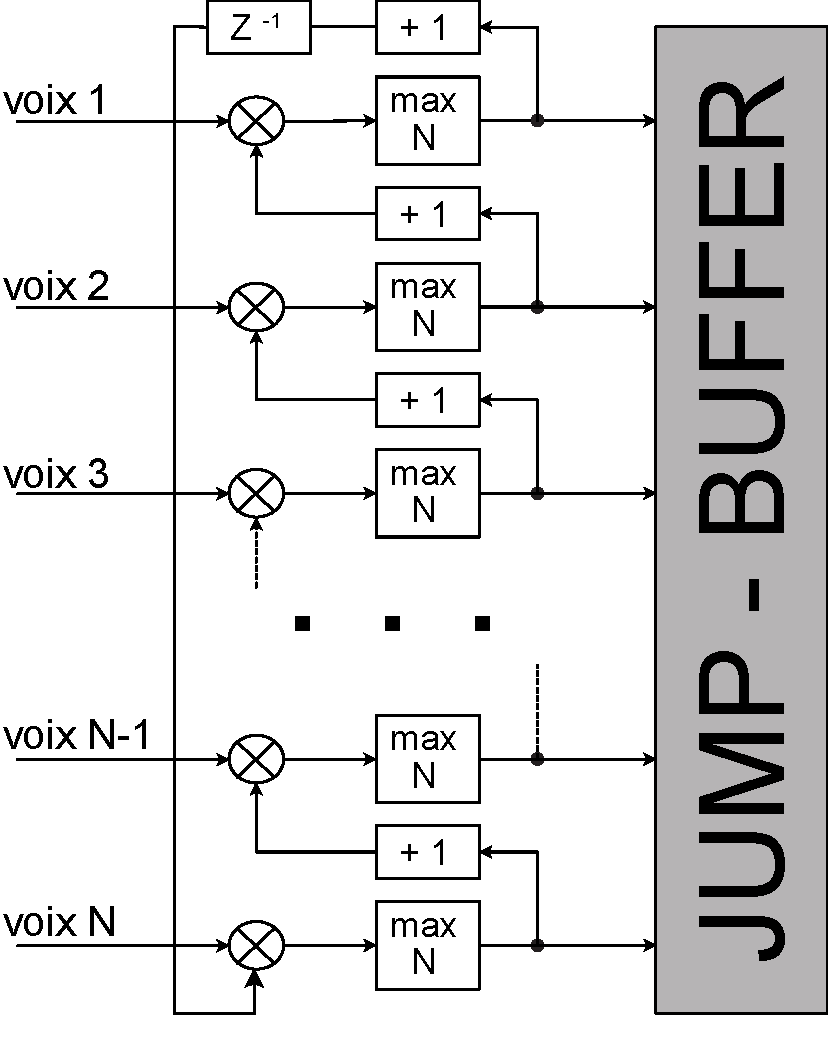
\includegraphics[width=\textwidth]{gfx/04_algorithms/sagrada-jumpBuffer.pdf}
	\caption[Sagrada : schéma fonctionnel de la computation synchrone du \textit{jump-buffer}]{Schéma fonctionnel de la computation synchrone du \textit{jump-buffer}}
	\label{fig:algorithms:sagrada-jumpBuffer}
\end{figure}
%------------------ Figure : Sagrada-jump-buffer ---------------------

\subsubsection{Gestion des flux de grains}

\noindent Si l'on considère l'ensemble des grains générés comme un flux, se posent alors deux questions concernant leur gestion :
\vspace{-1em}
\begin{itemize}[noitemsep]
	\item \textbf{la gestion d'un flux dans sa durée} : concètement, si je considère un flux de grain comme un macro-objet temporel ayant un début et une fin, une gestion particulière des coupures de début et de fin est souhaitable pour adapter la nature du son à un niveau micro-temporel à la forme macro-temporelle (par exemple en choisissant un grain particulier pour l'attaque);
	\item \textbf{la gestion de la multiplicité des flux} : concrètement, et pour faire le lien avec les développements présentés dans MP, si un doigt peut contrôler un flux de grains, un autre doigt doit pouvoir contrôler un autre flux de grains (et ainsi de suite) sans qu'il y ait de confusion dans le contrôle de chacun de ces flux.
\end{itemize}

\noindent La gestion de flux de grains est prise en charge par l'objet \verb|sagrada.multilayer~| (figure \ref{fig:algorithms:MP-multilayers}), qui permet de multiplexer plusieurs horloges en leur attribuant un index. Cet index de flux permet le décompte des grains par flux et en particulier, d'utiliser cet index pour gérer des grains individuels tels que le premier et le dernier grain d'un flux, qui peuvent ainsi être sélectionnés pour l'attaque et extinction du son.\\
\indent Un mécanisme de feedback interne permet d'éviter le conflit potentiel entre plusieurs \textit{ticks} d'horloge qui seraient déclenchés exactement au même instant (i.e. sur le même échantillon d'un signal). Dans ce cas précis, la priorité est donnée au flux de plus haut niveau\footnote{c'est-à-dire concrètement à celle gérée dans la voix de polyphonie la plus élevée de l'objet poly\textasciitilde{} gérant les différents flux.} Toutefois, ce cas de figure étant peu probable statistiquement, le multiplexage permet de n'utiliser qu'un seul et unique signal \gls{MSP} pour la gestion de l'ensemble des flux et d'économiser ainsi en ressources \gls{CPU}.\\
\indent Cette gestion de la polyphonie des flux de grains permet de les contrôler facilement avec des messages MP, comme le montre l'exemple sur la figure \ref{fig:algorithms:MP-and-Sagrada}, qui implémente un contrôle des flux de grains via une tablette \textit{multitouch}. Chaque doigt peut ici déclencher un flux et en contrôler la hauteur des grains ainsi que leur fréquence sur les axes X et Y de la tablette.

%------------------ Figure : Sagrada-multilayers ---------------------
\begin{figure}[!htbp]
	\captionsetup{format=plain}
	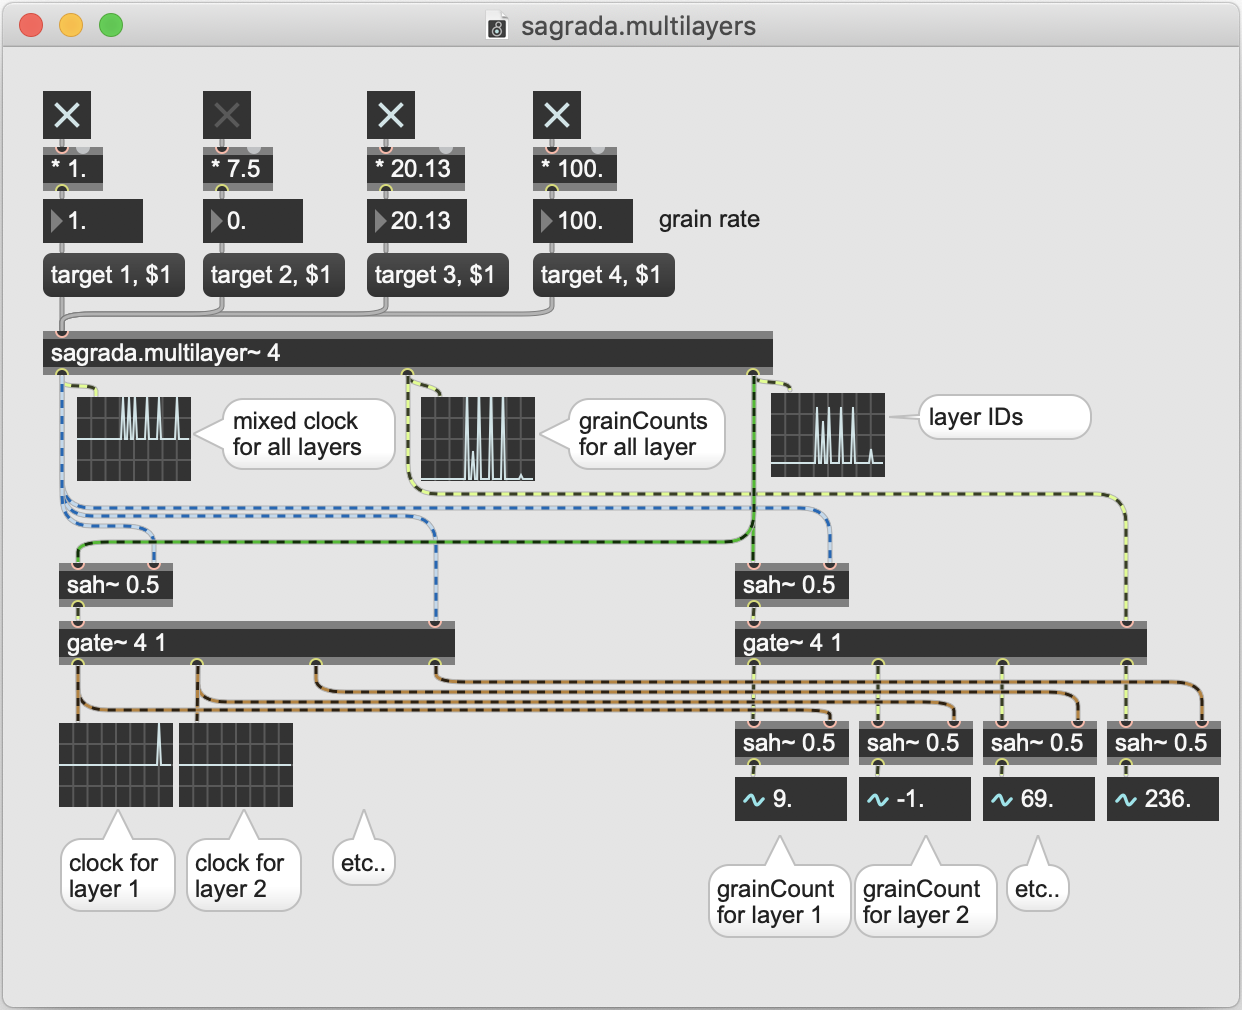
\includegraphics[width=\textwidth]{gfx/04_algorithms/Sagrada-multilayers.png}
	\caption[Sagrada : gestion de flux de grains]{Gestion de flux de grains par multiplexage d'horloges.}
	\label{fig:algorithms:MP-multilayers}
\end{figure}
%------------------ Figure : Sagrada-multilayers ---------------------

%------------------ Figure : mp-and-sagrada ---------------------
\begin{figure}[!htbp]
	\captionsetup{format=plain}
	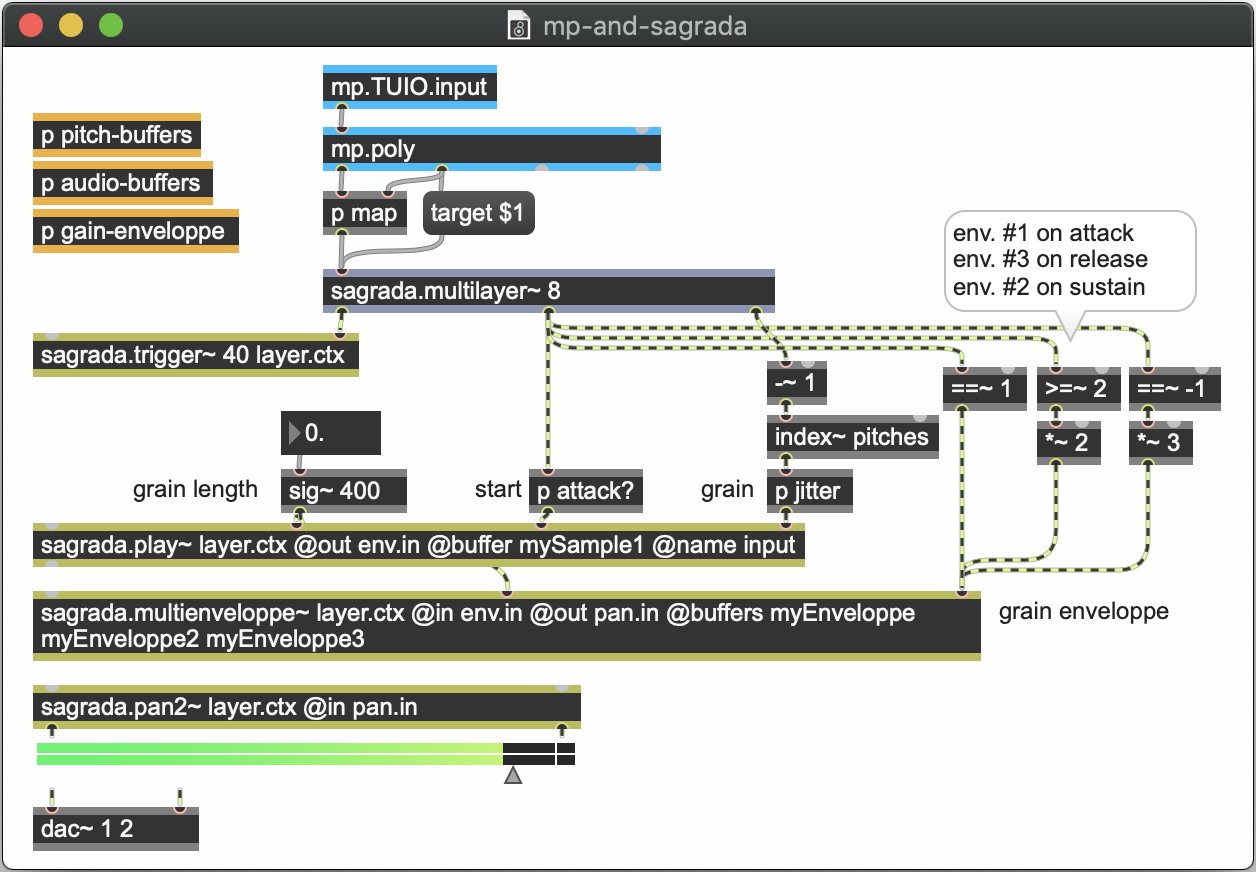
\includegraphics[width=0.5\textwidth]{gfx/04_algorithms/mp-and-sagrada.png}
	\caption[Contrôle de flux Sagrada avec MP]{Contrôle de flux Sagrada en multitouch, via MP.}
	\label{fig:algorithms:MP-and-Sagrada}
\end{figure}
%------------------ Figure : mp-and-sagrada ---------------------



%--------------------------------------------------------------
\subsection{Performances comparée}

\noindent L'avantage principal de Sagrada est de pouvoir composer une synthèse granulaire \textit{ad hoc} en traitant chaque grain de la manière souhaitée. En adoptant un système de déclenchement des grains via un signal \gls{MSP}, Sagrada bénéficie des mêmes avantages que le système \gls{GMU} (présentés dans \cite{bascou_gmu_2005}), en particulier la possibilité de ré-utiliser les systèmes de déclenchement stochastiques de grains fournis dans \gls{GMU}\footnote{Une réimplémentation partielle en a été faite dans la LAM-lib, notamment sa fonction de probabilité à densité [rand\_dist\_list\textasciitilde{}] dans l'objet [LAM.pdf\textasciitilde{}]}. Un avantage d'utiliser des impulsions par rapport au \textit{zéro-crossing} utilisé dans GMU est de diminuer de moitié (un échantillon au lieu de deux) l'intervalle entre deux grains successifs et de faciliter un déclenchement des grains par signaux d'horloges concurrentes\footnote{La raison en est que plusieurs trains d'impulsions \textit{s'additionnent} simplement (en limitant le signal crête à 1)}.\\
\indent Cependant, cette modularité implémentée dans le langage Max a un coût. À nombre de voix actives égales, le système \gls{GMU} consomme trois fois moins de ressources \gls{CPU} que Sagrada.


gen\textasciitilde{ } OLA, granularized, ftm, mc.*

\section{Conclusion}



\section*{[extra material]}

la production de hauteur dans les instruments acoustiques est systématiquement liée à un phénomène de résonance, c'est-à-dire un phénomène de bouclage, de feedback. 

La sélection de différentes hauteurs peut ensuite être obtenue 
- en jouant sur une multitude d'éléments accordés différemment (les cordes d'une harpe, les lames
d'un marimba, etc.) ;
- en modifiant les caractéristiques d'un élément résonnant, le plus souvent sa longueur (tube des
instruments à vent, corde d'un violoncelle) ;
- en sélectionnant des harmoniques précis d'un son riche (didgeridoo, chant diphonique).


Dans les DMIs la production de hauteur est essentiellement possible de deux manières: 
- par la lecture, éventuellement en boucle, d'une table d'onde
- par le délai de réinjection d'un filtre résonnant (synthèse soustractive, Karplus, etc.)
- par un calcul mathématique impliquant des fonctions périodiques (telles que les sinus dans la FFT).

L'acoustique physique présente naturellement des non-linéarités qui contribuent à la richesse du son et l'identité de son timbre. L'électronique analogique permet également d'obtenir --~sur l'espace restreint d'un signal mono-dimensionnel par rapport à l'acoustique physique généralement bi- ou tri-dimensionnelle~-- des systèmes résonants non-linéaires et stables, via l'utilisation de composants électroniques passifs.

Les choses sont plus compliquées pour le son numérique, s'il est possible d'obtenir des systèmes résonants stables (en maintenant les pôles dans le cercle unitaire du plan complexe), la garantie de stabilité devient très complexe à évaluer dès que l'on introduit de la non-linéarité.
Malgré de récentes avancées dans ce domaine (cf. travaux de Thomas Hélie sur les systèmes Hamiltoniens à ports)

